\chapter{Optical pumping of an atom laser}
\label{OpticalPumping}
\graphicspath{{Figures/OpticalPumping/}{Figures/Common/}}

The results presented in this chapter have been published in~\citet{Robins:2008,Doring:2009}.

\section{Motivation}

The development of the continuous-wave optical laser was a significant advance over the first pulsed ruby laser. The continuous-wave optical laser opened up many applications. The atom laser is a very promising source for both precision measurement and fundamental physics.

The replenishment process can be divided into two critical components: a delivery system for filling an atomic reservoir with ultracold atoms and a pumping mechanism for irreversibly and continuously transferring atoms from the reservoir to the laser mode.

The technical requirements on both parts of the replenishment system are stringent. Nonetheless, recent experiments have demonstrated that a delivery system for atoms is feasible and possible.~\citet{Chikkatur:2002qa} showed that Bose-condensed atoms could be periodically transported over large distances using a moving optical dipole trap. Further experiments with transport, based on interference of two counter-propagating lasers, have shown that dipole trapping techniques could be extended to provide continuous delivery of atoms~\citep{Schmid:2006}. Magnetic guiding systems for ultracold atoms may also provide a path to future delivery systems~\citep{Lahaye:2004,Greiner:2001,Greiner:2007}.

The realisation of the pumping mechanism for a continuous atom laser has proved more problematic. There are four critical requirements that are difficult to satisfy experimentally. First, the atoms should enter the laser mode continuously and coherently, that is, with the phase and amplitude of the lasing condensate. Thus, atoms must make a transition that is Bose-stimulated by the atomic lasing mode. The second requirement is that the pumping process is irreversible. It requires coupling to a reservoir. There are two reservoirs available, the empty modes of the electromagnetic field accessible via a transition from an excited atomic state, or the empty modes of the atomic field accessible via evaporation. For a high-coherence atom laser, the lasing mode must be a pure condensate with a significantly smaller thermal fraction, making evaporation-induced pumping a difficult possibility for the production for a highly coherent continuous atom laser. The third requirement is that the pumping system must be compatible with a continuous replenishment mechanism. This suggests strongly that there be a physical separation between the source and the lasing condensates. A physical separation with a stimulated transition between the source and the lasing mode isolates the lasing mode from phase kicks and heating that would result either as a necessary consequence of the replenishment system (for example in the replenishment system demonstrated by~\citet{Chikkatur:2002qa} where condensates are merged) or as a consequence of an imperfect delivery system. Finally, the fourth condition on a pumping system is that it should be possible to continuously output-couple atoms from the laser mode into a beam, while the pumping mechanism is operating.

The two possibilities for reservoirs to supply the irreversibility necessary for the proper operation of a pumped atom laser (Bose-Einstein condensate) are considered in this chapter and the next. In this chapter, pumping an atom laser using interactions mediated by light is considered. In this case the reservoir providing the irreversibility are the vacuum electromagnetic modes into which light is scattered by the pumping process. \chapterref{KineticTheory} considers the alternate possibility of using atomic \emph{s}-wave scattering interactions to mediate the pumping process with evaporation to make the process irreversible.

\hrule

Previous work on light-BEC interactions. Rayleigh/Raman superradiance, EIT, CARL, and the rest of that list that I had.


\section{Pumping mechanism}
\label{OpticalPumping:PumpingMechanism}

\begin{figure}
    \centering
    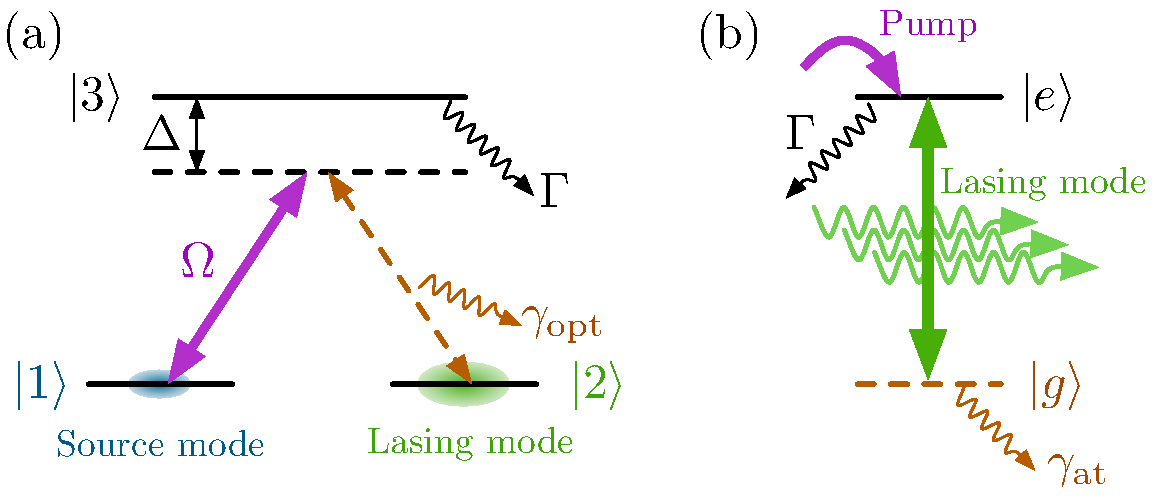
\includegraphics[width=14cm]{AtomLaserVsOpticalLaser}
    \caption{FIXME: This is not a caption. Comparison of considered atom laser pumping scheme (a) and typical optical laser pumping scheme (b).\label{OpticalPumping:AtomLaserVsOpticalLaser}}
\end{figure}

The optical pumping process under investigation in this chapter is illustrated in \figureref{OpticalPumping:AtomLaserVsOpticalLaser}(a).  In this process atoms in the source mode are driven by a laser into an excited state from which they can decay into the lasing mode (the condensate).  Although there is no laser driving this second transition ($\ket{3}\leftrightarrow\ket{2}$), the decay of atoms into the lasing mode is not spontaneous emission in the usual sense.  The emission process is \emph{atomically}-stimulated by the large occupation of the lasing mode in the same way that the transition may be \emph{optically}-stimulated even in the absence of any population in the atomic state into which the atom decays.

The final decay of an atom into the lasing mode in \figureref{OpticalPumping:AtomLaserVsOpticalLaser} resembles standard \emph{optical} laser schemes [see \figureref{OpticalPumping:AtomLaserVsOpticalLaser}(b)] in which the roles of atoms and light are reversed.  In an optical laser an atom in the excited state is stimulated to emit into the ground state by the resonant photons in the laser cavity.  Once the atom has emitted, it decays rapidly into other internal states with rate $\gamma$ significantly limiting reabsorption from the $\ket{g}$ state.  A similar process occurs in the proposed optical pumping scheme in which the photon emitted as the atom decays  leaves the system rapidly preventing reabsorption.  The loss of photons from the system is represented by the decay of the optical mode with rate $\gamma$ in \figureref{OpticalPumping:AtomLaserVsOpticalLaser}(a).

This similarity between the proposed atom laser pumping mechanism and the usual optical laser pumping mechanism is clearly illustrated by considering the Hamiltonian coupling the excited and ground atomic states in \figureref{OpticalPumping:AtomLaserVsOpticalLaser}
\begin{align}
    \hat{H} &= \hbar \epsilon \left(\hat{a}_e^\dagger \hat{a}_g \hat{a}_\text{ph} + \hat{a}_g^\dagger \hat{a}_\text{ph}^\dagger \hat{a}_e  \right),
    \label{OpticalPumping:TwoLevelAtomHamiltonian}
\end{align}
where $\epsilon$ is a real coupling constant, the $\hat{a}_e$, $\hat{a}_g$, and $\hat{a}_\text{ph}$ are annihilation operators for the atomic excited state, atomic ground state and photon mode respectively.  The rotating wave approximation has been made in obtaining this Hamiltonian, assuming that the optical mode is not detuned from the atomic transition by a large fraction of the frequency difference between the two states.  

The Hamiltonian \eqref{OpticalPumping:TwoLevelAtomHamiltonian} describes both the atom- and optical-laser pumping mechanisms, the difference in the mechanisms being in the occupations of the various states.  If the system is initially in a state with $N_e$ atoms in the atomic excited state, $N_g$ atoms in the atomic ground state and $N_\text{ph}$ photons in the optical mode, the amplitude for an atom in the excited state to emit a photon is
\begin{align}
    \bra{N_e-1, N_g + 1, N_\text{ph} + 1} \hat{H} \ket{N_e, N_g, N_\text{ph}} &= \hbar \epsilon \sqrt{N_g+1} \sqrt{N_\text{ph}+1} \sqrt{N_e}.
\end{align}
This emission process can therefore be stimulated either by photons ($N_\text{ph} > 0$) or by atoms ($N_\text{g} > 0$).  It would also be possible for the emission to be stimulated by both photons \emph{and} atoms, although in this case the amplitude for the absorption process would be non-zero
\begin{align}
    \bra{N_e+1, N_g - 1, N_\text{ph} - 1} \hat{H} \ket{N_e, N_g, N_\text{ph}} &= \hbar \epsilon \sqrt{N_e+1} \sqrt{N_\text{ph}} \sqrt{N_g}.
\end{align}
It is for this reason that it is desirable in an optical laser to have $N_g \approx 0$, and in the proposed atom laser pumping scheme to have $N_\text{ph} \approx 0$.

Atom laser pumping schemes of the form of that illustrated in \figureref{OpticalPumping:AtomLaserVsOpticalLaser}(a) have been proposed before~\citep{Olshanii:1996,Janicke:1996,Spreeuw:1995,Cirac:1996rr,Cirac:1996,Santos:2000,Castin:1998,Cirac:1994,Vengalattore:2003,Santos:2001ve,Wolf:2000,Santos:1999qf} for the production of BEC without the use of collisional evaporation and its consequent losses.  The main problem that they all seek to address is that of reabsorption of photons spontaneously emitted when the atom in state $\ket{3}$ decays to the $\ket{2}$ state, but not to the lasing mode.  This emitted photon will be resonant with the lasing mode and may be scattered several times before finally leaving the condensate.  A single such spontaneously emitted photon can cause significant heating of a condensate as the single photon recoil energy can be as large as or greater than the chemical potential of the condensate.

One proposed method~\citep{Castin:1998,Vengalattore:2003} for reducing the heating uses a purely geometric solution: if a condensate is made sufficiently narrow in one or more dimensions such that a photon emitted in one of those directions is negligibly likely to be reabsorbed, the overall probability for reabsorption will also be reduced.  While this method may be appropriate for the initial formation of BEC, it is impractical for a large BEC as the trap deformation necessary to reach the required regime is extreme.  For a \nucl{87}{}{Rb} condensate of $N= 5\times 10^5$ atoms with trapping frequencies of $\omega_x = \omega_y = \unit[2\pi \times 128]{Hz}$, $\omega_z = \unit[12.8]{Hz}$, the mean-free path in the centre of the condensate for a resonant photon on the cycling transition ($\lambda = \unit[780]{nm}$) is $1/(n \sigma) = \unit[16]{nm}$ where $n$ is the peak condensate density and $\sigma = 3 \lambda^2/2 \pi$ is the atomic scattering cross-section.

Another possibility for reducing reabsorption that works well in optical lattices is to operate in the \emph{festina lente} regime~\citep{Wolf:2000,Santos:1999qf,Cirac:1996,Castin:1998} in which the energy levels of the trap are sufficiently separated such that a photon emitted when an atom decays into a particular trap level is only resonant with atoms in that level (and those levels degenerate with it).  This prevents the occurrence of `dangerous' processes in which an excited atom decays into a non-condensate level with the emitted photon being absorbed by the condensate.  In the case of resonant optical pumping light ($\Delta = 0$ in \figureref{OpticalPumping:AtomLaserVsOpticalLaser}(a)), the \emph{festina lente} regime requires that $\omega_\text{min} \gg \Gamma$  where $\omega_\text{min}$ is the minimum of the magnetic trapping frequencies.  Strictly, the \emph{festina lente} regime has only been investigated in the absence of \emph{s}-wave scattering interactions, however one would expect that in the presence of \emph{s}-wave scattering the trap frequency energy scale would simply be replaced by the energy of the relevant Bogoliubov excitation (refer to \sectionref{Peaks:ElementaryExcitations}).  Regardless, the \emph{festina lente} regime is impractical to achieve in alkali gases like \nucl{87}{}{Rb} as the relevant decay rate is $\Gamma = \unit[2\pi\times 5.9]{MHz}$, which is much larger than typical trap frequencies ($\omega \sim \unit[2\pi \times 100]{Hz}$) and condensate excitations ($\mu/\hbar \sim \unit[2\pi \times 10]{kHz}$).

A third possibility for reducing reabsorption is to operate in the \emph{boson accumulation regime} (BAR)~\citep{Cirac:1996rr,Floegel:2001} in which an atom in the excited state is significantly more likely to decay into the condensate mode than into all other modes.  In this limit it can be shown that absorption of emitted photons by atoms not in the condensate mode can be neglected.  It is in the BAR that we wish to operate our proposed pumping mechanism of \figureref{OpticalPumping:AtomLaserVsOpticalLaser}(a).  

Up to this point, the source mode was entirely arbitrary; without consideration of reabsorption the proposed pumping process would work equally well for coherent or thermal states in the source mode.  As the optical transition between the excited atomic state and the lasing mode is not driven by a laser, the phase of the photons emitted is determined by the relative phase between the source and lasing modes; the direction of population transfer does not depend on the phase difference between these two modes. However the requirement that excited atoms be significantly more likely to decay into the condensate mode than to any other mode places a stringent requirement on the source mode of the pumping mechanism.  For this requirement to be satisfied, the momentum width of the source atom distribution cannot be significantly larger than the momentum width of the condensate.  If this were not the case a significant fraction of the atoms would not be momentum-resonant with the condensate under the pumping process and will therefore not be in the boson accumulation regime.  These atoms would be able to reabsorb spontaneously emitted photons causing the reabsorption problem previously discussed.  For an atomic distribution to have a momentum width comparable to that of the target condensate, the atoms must either be condensed or if they are thermal, be trapped in a significantly weaker trap than the target condensate mode and have a temperature below the condensation temperature in the tighter trap.  

Although it would be desirable to be able to use a thermal source of atoms as the source mode, the remainder of this chapter will investigate the possibility of using a coherent source of atoms as the source mode of the pumping mechanism.  Specifically, this coherent source will be an atom laser extracted from a second, source condensate.  Continuous operation of this scheme could in principle be achieved by replacing the source condensate with an independently-produced condensate once it is depleted.  As the pumping mechanism is independent of the phase-difference between the source and lasing modes this will not affect the direction of population transfer.

% \parasep
% 
% The pumping mechanism described in this section bears some resemblance to other optical processes that can occur in Bose-Einstein condensates such as EIT, and Rayleigh/Raman superradiance. FIXME: Complete paragraph/s.
% 
% Quote from the paper:
% 
% The mechanism we have described for pumping is related to pulsed Raman super-radiance that has been studied previously.  In our work, in the laboratory frame, atoms are driven from the $\ket{2, 0}$ untrapped state into the $\ket{1, -1}$ trapped state enabling us to continue pumping indefinitely.  the condensate that we pump is stationary in the laboratory frame.  Furthermore, our experiment is carried out in a double-condensate geometry with internal states that enable simultaneous pumping and outcoupling to produce a freely propagating atom laser beam from a simultaneously pumped condensate.
% 
% There is a second mechanism that we have considered that is related to the EIT mechanism described in the work by~\citet{Ginsberg:2007fk}.  Similar to the existing Raman super-radiance experiments, their work was necessarily carried out in a pulsed regime.  In our experiment, again, the geometry and choice of internal states enable the possibility of carrying out a related experiment continuously.  The condensates in such an experiment must have some spatial overlap.  The $\ket{2, 0}$ atoms are produced in the overlap region where the $\pi$-polarised pump beam is absorbed and the $\sigma$-polarised beam is produced.  Both beams travel in the same direction.  The amplitude of the $\pi$-polarised beam decays in the overlap region.  The amplitude of the $\sigma$-polarised beam grows.  The atoms follow the dark state and are pumped continuously to the lasing mode.


\section{The continuous pumping experiment}
\label{OpticalPumping:ContinuousExperiment}

A summary is provided here of the continuous pumping experiment performed by \emph{Nick Robins}, \emph{Cristina Figl} and \emph{Matthew Jeppesen} at the Department of Quantum Science, ANU.  Further details of the experimental setup and results are published in \citet{Robins:2008}.

\begin{figure}
    \centering
    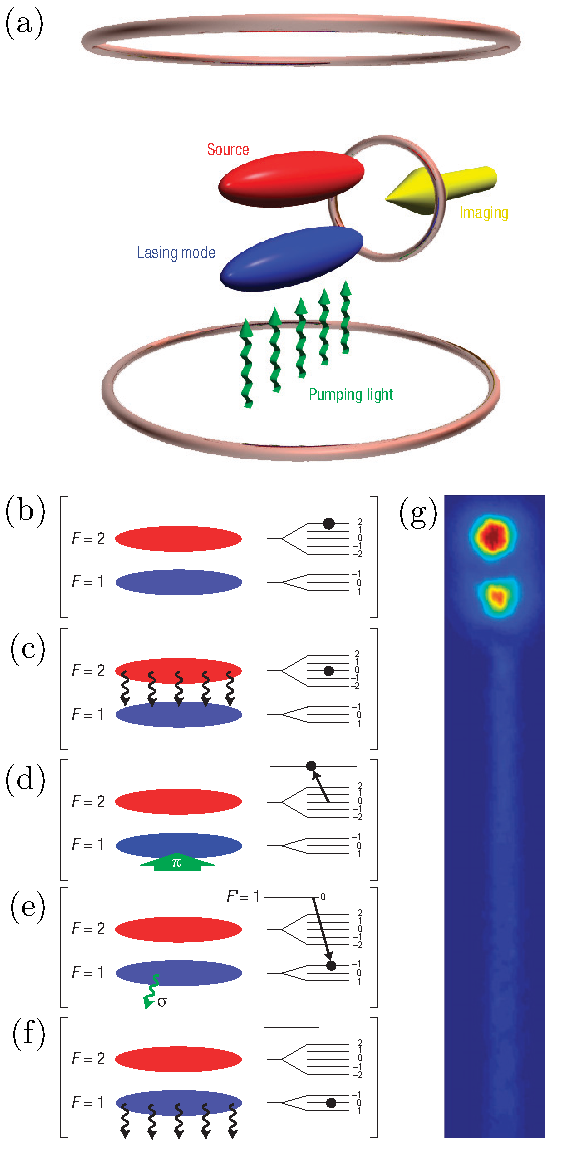
\includegraphics[width=8cm]{ExperimentSchematic}
    \caption{FIXME: Caption.  Schematic diagram of the operation of the pumped atom laser.  Schematic diagram of the experiment (a) and pumping steps (b--f).  A radiofrequency field spin-flips the atoms to the $\ket{2, 0}$ state (b), and they fall under gravity (c).  The light field couples the atoms to the $F'=1$ excited state from which they are stimulated to emit into the $\ket{1, -1}$ BEC.  The atomic momentum is cancelled by the absorption and emission of the photons (d, e).  A second radiofrequency field finally output-couples the atoms into the $\ket{1, 0}$ atom laser (f).  (g), Absorption image of the experimental system, showing source, laser mode and output beam.}
    \label{OpticalPumping:ExperimentSchematic}
\end{figure}

\begin{table}
    \centering
    \begin{tabular}{cc}
    \toprule
    Parameter & Value\\
    \midrule
    $\ket{F=2, m_F=2}$ (source) condensate number & $N_\text{source} = (6.7 \pm 0.5)\times 10^5$ \\
    $\ket{F=1, m_F=-1}$ (laser) condensate number & $N_\text{laser} = (5.0 \pm 0.4) \times 10^5$ \\
    Radial trapping frequency (for $\ket{1, -1}$) & $\omega_r = \unit[2\pi \times 130]{Hz}$ \\
    Axial trapping frequency (for $\ket{1, -1}$) & $\omega_z = \unit[2\pi \times 13]{Hz}$ \\
    \bottomrule
    \end{tabular}
    \caption{Experimental parameters for the Rubidium-87 BEC system under consideration.}
    \label{OpticalPumping:ExperimentalParameters}
\end{table}


To produce a pumped atom laser two independent condensates are prepared in the $\ket{F=2, m_F=2}$ and $\ket{F=1, m_F=-1}$ magnetically trapped states of \nucl{87}{}{Rb}.  Owing to their larger magnetic moment, the $\ket{2, 2}$ atoms are more tightly confined in the magnetic field than the $\ket{1, -1}$ atoms, and hence the evaporation does not directly cool them.  They are, however, sympathetically cooled through elastic collisions with the $\ket{1, -1}$ atoms~\citep{Myatt:1997}.  For the condensate numbers and trapping frequencies given in \tableref{OpticalPumping:ExperimentalParameters} the Thomas-Fermi radius of each cloud is approximately $\unit[5]{\micro m}$ in the vertical direction.  The different magnetic moments of the two clouds lead to a gravitational sag between their centres of $\unit[8]{\micro m}$. Hence, the two clouds of atoms overlap only slightly, with the $\ket{2, 2}$ source condensate located above the $\ket{1, -1}$ laser-mode condensate [see \figureref{OpticalPumping:ExperimentSchematic}(a)].

To measure the effect of pumping, it is essential that the number of atoms in each state is stable from one experimental run to the next.  For this purpose, many details of the apparatus were refined, including very efficient baffling against stray resonant light, very low uncertainty and drift in laser frequency, intensity and polarisation, and good vibrational and thermal stability of the trap.  The stability of the number of atoms in each state was determined for a data set comprising 20 measurements, and found to be as low as 1\%.

The operation of the experiment is illustrated in \figureref{OpticalPumping:ExperimentSchematic}.  Starting with an initial number of atoms in each state [\figureref{OpticalPumping:ExperimentSchematic}(b)], a weak continuous radiofrequency field is applied to the upper source cloud which couples atoms from the $\ket{2, 2}$ state, through $\ket{2, 1}$ to the $\ket{2, 0}$ state.  This coupling is highly spatially selective and does not affect the $\ket{1, -1}$ cloud.  These atoms begin to fall away from the $\ket{2, 2}$ source cloud [\figureref{OpticalPumping:ExperimentSchematic}(c)].  Simultaneously approximately $\unit[10]{pW}$ of upward propagating $\pi$-polarised light resonant with the $\ket{F=2}\rightarrow\ket{F'=1}$ transition is applied.  Although this light is resonant in energy with the $\ket{2, 2}$ source atoms, they are prevented from absorbing photons by atomic selection rules.  Hence, the source cloud is unaffected by the pumping light.  For pumping the laser mode, the $\ket{2, 0}$ atoms will absorb the pumping light [\figureref{OpticalPumping:ExperimentSchematic}(d)].  As these atoms fall, they may make a transition into the excited $\ket{F'=1, m_F=0}$ state from which they are stimulated to emit into the laser mode $\ket{1, -1}$ by the atoms already present in that mode [\figureref{OpticalPumping:ExperimentSchematic}(e)].  The $\sigma^{+}$-photon emitted in this process carries the phase difference between the pump atoms and the condensate.  Finally, the $\ket{1, -1}$ laser-mode atoms are output-coupled to produce the atom laser beam in the $\ket{1, 0}$ state [\figureref{OpticalPumping:ExperimentSchematic}(f)].  An absorption image of the ultracold atoms used to build the pumped atom laser system is shown in \figureref{OpticalPumping:ExperimentSchematic}(g).

For successful pumping, the pump atoms must be momentum-resonant with the lasing condensate.  This means that their atomic velocity after the emission of the photon has to lie within the velocity spread of the BEC.  The magnetic trapping frequencies were chosen not only to position the two clouds as closely as possible without significant overlap, but also such that the velocity acquired by a $\ket{2, 0}$ atom in falling from the centre of the $\ket{2, 2}$ cloud to the centre of the $\ket{1, -1}$ laser mode ($\unit[12]{mm\, s\textsuperscript{-1}}$) can be cancelled by the absorption of an appropriately directed and phased $\sigma^{+}$-photon; a single-photon recoil corresponds to $\unit[6]{mm\, s\textsuperscript{-1}}$.  The velocity at the laser-mode centre can be tuned by around $\unit[\pm 2]{mm\, s\textsuperscript{-1}}$ by moving the coupling surface within the source cloud up or down.  While the pump atoms are falling through the $\ket{1, -1}$ laser mode, the velocity varies by $\unit[\pm 3]{mm\, s\textsuperscript{-1}}$ owing to gravity and the time for which the pumping atoms satisfy momentum resonance with the laser mode is much shorter ($\sim \unit[100]{\micro s}$) than the traversal time across the laser mode ($\sim\unit[1]{ms}$).  The velocity spread of the laser mode is of the order of $\unit[0.3]{mm\, s\textsuperscript{-1}}$; thus, cancelling the atomic momentum of the $\ket{2, 0}$ state requires an extreme level of control over pumping parameters.  In the experiment no collective motion, such as sloshing or breathing of either the source- or laser-mode condensates was observed.  This implies that if excitations driven by the pumping exist, they occur with an amplitude of less than 5\% of the full-width at half-maximum of the laser-mode condensate, which was inferred from the resolution limit of the imaging system.

\begin{figure}
    \centering
    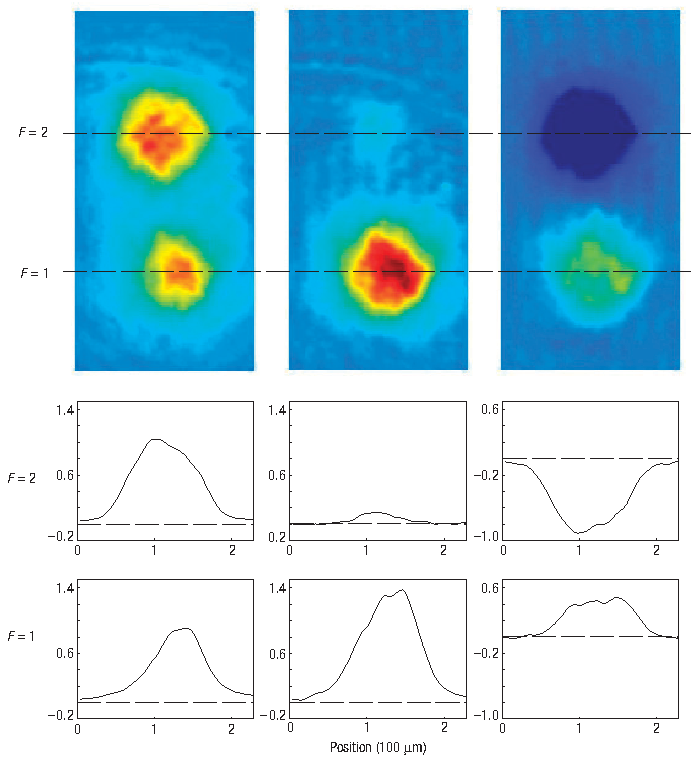
\includegraphics[width=12cm]{ExperimentalResults}
    \caption{FIXME: Caption.  Blue-detuned absorption images averaged over three identical runs of the experiment (top row); detuning of the probe laser from resonance is $\unit[7]{MHz}$.  The graphs below are horizontal cross-sections through the absorption images, showing optical depth, averaged over $\unit[50]{\micro m}$ in the vertical direction.  The tree columns correspond to: pumping off (left); pumping on (centre); difference between pumped and unpumped (right).}
    \label{OpticalPumping:ExperimentalResults}
\end{figure}

To isolate and study the pumping mechanism, the experiment was first operated without outcoupling from the laser-mode condensate.  \figureref{OpticalPumping:ExperimentalResults} demonstrates the effect \unit[200]{ms} of pumping has on the $\ket{1, -1}$ condensate; the left-hand image is taken without outcoupling from either condensate and without the pumping light.  The absorption image shows the unpumped $F=1$ laser-mode BEC (the lower cloud) with the $F=2$ source atoms above.  The curves below are horizontal cross-sections through the absorption images showing the optical depth of each atom cloud.  The central image shows the effect of \unit[200]{ms} of pumping on the laser-mode BEC.   The source is almost completely depleted and the laser-mode atom number has increased to $(7.2 \pm 0.4)\times 10^5$.  The third column shows the difference between the pumped and unpumped images. It is important to note that the profile of the laser-mode condensate after pumping has a significant Thomas-Fermi component with a small increase in the Gaussian thermal component.  The pumping efficiency, which is defined as the growth of the laser mode compared with the loss from the source, is $(35 \pm 10)\%$ for the results presented in \figureref{OpticalPumping:ExperimentalResults}.

A second experiment was also performed simultaneously pumping the laser-mode BEC and outcoupling from this condensate to demonstrate that the production of the atom laser could be operated independently of the pumping mechanism into the condensate.  In this chapter we focus on the results of the first experiment in which the pumping mechanism was studied.

\parasep

The continuous pumping experiment just described was designed to transfer $2 \hbar k$ of momentum to the falling pump atoms (by absorbing a photon of momentum $\hbar k$ going up and then emitting a photon of similar momentum directed downwards) as they are transferred to the laser-mode condensate.  However, there is a second way for the pump atoms to be momentum-resonant with the laser-mode condensate.  If the outcoupling surface for the upper condensate is towards the lower edge of the condensate the outcoupled atoms will be in close proximity to the laser-mode condensate immediately below due to the slight spatial overlap.  These recently outcoupled atoms will have almost no momentum and will be able to absorb a $\pi$-polarised photon with momentum $\hbar k$ upwards and emit a $\sigma^+$-polarised photon of similar momentum also directed upwards, decaying into the lower laser-mode condensate with no net momentum transfer.

These two different processes are examined in greater detail theoretically in \sectionref{OpticalPumping:MultimodeModel}, however we begin our theoretical analysis of the experiment and the pumping mechanism more generally with a simple single-mode model of the process illustrated in \figureref{OpticalPumping:AtomLaserVsOpticalLaser}(a).


\section{Simple single-mode model}
\label{OpticalPumping:SingleModeModel}

We begin our theoretical investigation of the pumping mechanism behind the previously-described experiment by considering the simplest-possible model, a single-mode mean-field approximation to the process illustrated in \figureref{OpticalPumping:AtomLaserVsOpticalLaser}(a).  The equations of motion for this model are
\begin{subequations}
    \label{OpticalPumping:SingleModeModel}
    \begin{align}
        \frac{d}{dt} c_\text{source} &= -i \Omega^* c_\text{excited} \\
        \frac{d }{dt}c_\text{excited} &= -i \Omega c_\text{source} -i g \alpha c_\text{lasing} - i \Delta c_\text{excited} - \frac{\Gamma}{2} c_\text{excited}\\
        \frac{d }{dt}c_\text{lasing} &= -i g^* \alpha^* c_\text{excited} \\
        \frac{d }{dt}\alpha &= -i g^* c_\text{lasing}^* c_\text{excited}^{\phantom{*}} - \frac{\gamma}{2} \alpha,
    \end{align} 
\end{subequations}
where $c_\text{source}$, $c_\text{lasing}$ and $c_\text{excited}$ are the amplitudes of the source $\ket{1}$, lasing $\ket{2}$ and excited $\ket{3}$ modes respectively, $\Omega$ is the complex Rabi frequency due to the pumping laser coupling the source and excited modes with detuning $\Delta$, $\alpha$ is the amplitude of the optical mode into which the excited atoms emit when decaying into the lasing mode and $g$ is the complex coupling constant for this transition.  The optical mode $\alpha$ will decay as photons propagate away from the system.  This process is modelled phenomenologically with a loss rate $\gamma$ from the optical mode $\alpha$.  The spontaneous decay of the excited state into modes other than the lasing mode occurs at a rate $\Gamma$.  It has been assumed that the pumping laser is sufficiently strong to be negligibly absorbed.  This assumption is relaxed in \sectionref{OpticalPumping:MultimodeModel}.  The evolution equations \eqref{OpticalPumping:SingleModeModel} are given in a rotating frame in which the energy difference between the source, excited and lasing modes have been appropriately removed.

In deriving \eqref{OpticalPumping:SingleModeModel} it has been assumed that atoms that undergo spontaneous decay from the excited mode will have no further impact upon the system.  In particular this means that the absorption of photons in the $\alpha$ mode by atoms in modes other than the lasing mode has been neglected.  The absorption of these photons by the lasing mode is, however, retained.  As discussed in \sectionref{OpticalPumping:PumpingMechanism} this is a valid approximation in the boson accumulation regime in which an excited atom is significantly more likely to decay into lasing mode than into any other mode.

The long-term dynamics of \eqref{OpticalPumping:SingleModeModel} will determine the usefulness of the process as a pumping mechanism.  The fast-timescale behaviour of this system can therefore be eliminated.  By far the fastest process in the system is the decay of the photons in the $\alpha$ mode as they leave the system.  The time taken for a photon to cross the width of a typical condensate ($\sim\unit[10]{\micro m}$) is $\sim\unit[10^{-13}]{s}$, giving $\gamma \sim \unit[10^{13}]{s\textsuperscript{-1}}$.  By comparison, the spontaneous decay rate of the excited mode is $\Gamma \sim \unit[10^8]{s\textsuperscript{-1}}$ for the $F'=1$ manifold of \nucl{87}{}{Rb}.  As the $\alpha$ mode reaches a quasistationary value on the fastest timescale in the system ($\gamma$), it can be adiabatically eliminated and replaced with its quasistationary limit,
\begin{align}
    \alpha & \approx -\frac{2 i g^*}{\gamma} c_\text{lasing}^* c_\text{excited}. \label{OpticalPumping:Alpha}
\end{align}

We next assume that the pump laser is driving the atoms in the weak-field regime, $\Omega \ll \max\left(\Delta, \Gamma\right)$.  In this limit, the excited mode $c_\text{excited}$ evolves on a more rapid timescale than either the source or lasing modes.  The excited mode may therefore also be adiabatically eliminated and replaced with its long-term average
\begin{align}
    c_\text{excited} &\approx \frac{-i \Omega c_\text{source}}{\frac{1}{2}\Gamma + 2 \frac{\abs{g}^2}{\gamma} N_\text{lasing} + i \Delta}, \label{OpticalPumping:CExcited}
\end{align}
where $N_\text{lasing} = \abs{c_\text{lasing}}^2$ is the number of atoms in the lasing mode.

With these two adiabatic eliminations made, the rate equations for the populations of the remaining two modes are obtained by substituting \eqref{OpticalPumping:Alpha} and \eqref{OpticalPumping:CExcited} into \eqref{OpticalPumping:SingleModeModel},
\begin{subequations}
    \label{OpticalPumping:SingleModeRateEquations}
    \begin{align}
        \frac{d}{dt} N_\text{source} &= - \frac{\abs{\Omega}^2 \left(\Gamma + \Gamma'\right)}{\abs{\frac{1}{2}(\Gamma + \Gamma') + i \Delta}^2} N_\text{source}\\
        \frac{d}{dt} N_\text{lasing} &= \frac{\Gamma'}{\Gamma + \Gamma'} \left( - \frac{d}{dt} N_\text{source}\right),
    \end{align}
\end{subequations}
where $\displaystyle \Gamma' = 4 \frac{\abs{g}^2}{\gamma} N_\text{lasing}$ is the rate constant with which atoms in the excited mode decay into the lasing mode.

The efficiency of the transfer of atoms in the pumping process is $\Gamma'/(\Gamma + \Gamma')$, which behaves as expected: as the occupation of the lasing mode $N_\text{lasing}$ is increased, the efficiency increases due to bosonic stimulation.  What is perhaps not expected is the behaviour of the transfer rate constant.  In the limit of large detuning, $\Delta \gg \Gamma + \Gamma'$, the rate constant for atom transfer is
\begin{align}
    \left.-\frac{d}{dt} N_\text{source}\middle/N_\text{source}\right. &\approx \frac{\abs{\Omega}^2}{\Delta^2} \left(\Gamma + \Gamma'\right), \label{OpticalPumping:SingleModePumpingRateLargeDetuning}
\end{align}
which increases as the lasing mode population increases (due to increasing $\Gamma'$).  In the limit of small detuning however ($\Delta \ll \Gamma + \Gamma'$) very different behaviour is obtained
\begin{align}
    \left.-\frac{d}{dt} N_\text{source}\middle/N_\text{source}\right. &\approx 4 \frac{\abs{\Omega}^2}{\Gamma + \Gamma'}, \label{OpticalPumping:SingleModePumpingRateZeroDetuning}
\end{align}
which \emph{decreases} as the lasing mode population increases.  This behaviour is due to the depletion of the excited state as $\Gamma'$ increases.  In the limit of small detuning, spontaneous and stimulated decay are the fastest processes reducing the occupation of the excited state, hence increasing those rates will reduce the overall population of the excited state.  In this limit as the excited state population decreases proportional to the squared sum of these rates
\begin{align}
    N_\text{excited} &\approx 4 \frac{\abs{\Omega}^2}{(\Gamma + \Gamma')^2} N_\text{source},
\end{align}
the overall rate of atom transfer is suppressed as these processes occur on faster timescales.  In the opposite limit of large detuning, the spontaneous and stimulated decay processes are a perturbation on the Rabi-flopping process which populates the excited state.  In this limit the excited state population is independent of the spontaneous and stimulated emission rates
\begin{align}
    N_\text{excited} &\approx \frac{\abs{\Omega}^2}{\Delta^2} N_\text{source},
\end{align}
and the overall atom transfer rate into the lasing mode can be Bose-enhanced.

\parasep

The simple model developed in this section can be applied to the continuous pumping experiment described in \sectionref{OpticalPumping:ContinuousExperiment} to give a limit for the efficiency of the `$2 \hbar k$' momentum-transfer process.  In this process falling atoms outcoupled from the upper condensate reach a momentum of $2\hbar k$ vertically downwards before absorbing a pump photon of momentum $\hbar k$ from below and emitting a photon of similar momentum directed downwards to decay into the lasing mode.  If it is assumed that the intensity of the pump mode is approximately constant throughout the system, then the rate of transfer of atoms into the lasing mode cannot be faster than the rate of spontaneous emission while the source atoms are not momentum-resonant with the lasing mode\footnote{When the source atoms are not momentum-resonant with the lasing mode, it is equivalent to there being no atoms in the lasing mode.  In this case, $\Gamma'=0$ and from \eqref{OpticalPumping:SingleModePumpingRateZeroDetuning} it can be seen that the spontaneous emission rate must be greater than the transfer rate into the condensate.}.  An upper bound for the efficiency of the `$2 \hbar k$' momentum-transfer process should therefore be given by the ratio of the time for which the source atoms are momentum-resonant with the condensate ($\sim\unit[100]{\micro s}$, see \sectionref{OpticalPumping:ContinuousExperiment}) to the fall time for the atoms to that point ($\sim\unit[1]{ms}$).  As the upper bound for this process $(\sim 10\%)$ is lower than the observed efficiency $(\sim 35\%)$, either the transfer of atoms into the lasing mode must significantly reduce the intensity of the pump mode, or it must be the `$0 \hbar k$' process that operates in the continuous pumping experiment.  The argument used to obtain an upper bound for the efficiency of the `$2 \hbar k$' momentum-transfer process does not apply to the `$0 \hbar k$' momentum-transfer process in which atoms outcoupled from the upper condensate can be immediately pumped into the lower condensate.

The simple model considered in this section does not take into account the behaviour of the emitted photons in the $\alpha$ mode as they traverse the source and/or lasing modes as they leave the system.  The investigation of this and other multimode effects is the subject of the next section and will be shown to lead to modifications of the behaviour described by the simple single-mode model.

\section{Multimode model}
\label{OpticalPumping:MultimodeModel}

The multimode model we use in this chapter to describe the interaction of the BEC with the pumping light is similar to the Maxwell-Schrödinger equations \citep{Zobay:2005,Zobay:2006} used to describe superradiant Rayleigh scattering in BEC.  The difference here is that the pumping light may be much closer to resonance with the source atoms, and atoms can be stimulated to decay into a different internal atomic state from which they were excited (see the level diagram of \figureref{OpticalPumping:LevelDiagram}).

\begin{figure}
    \centering
    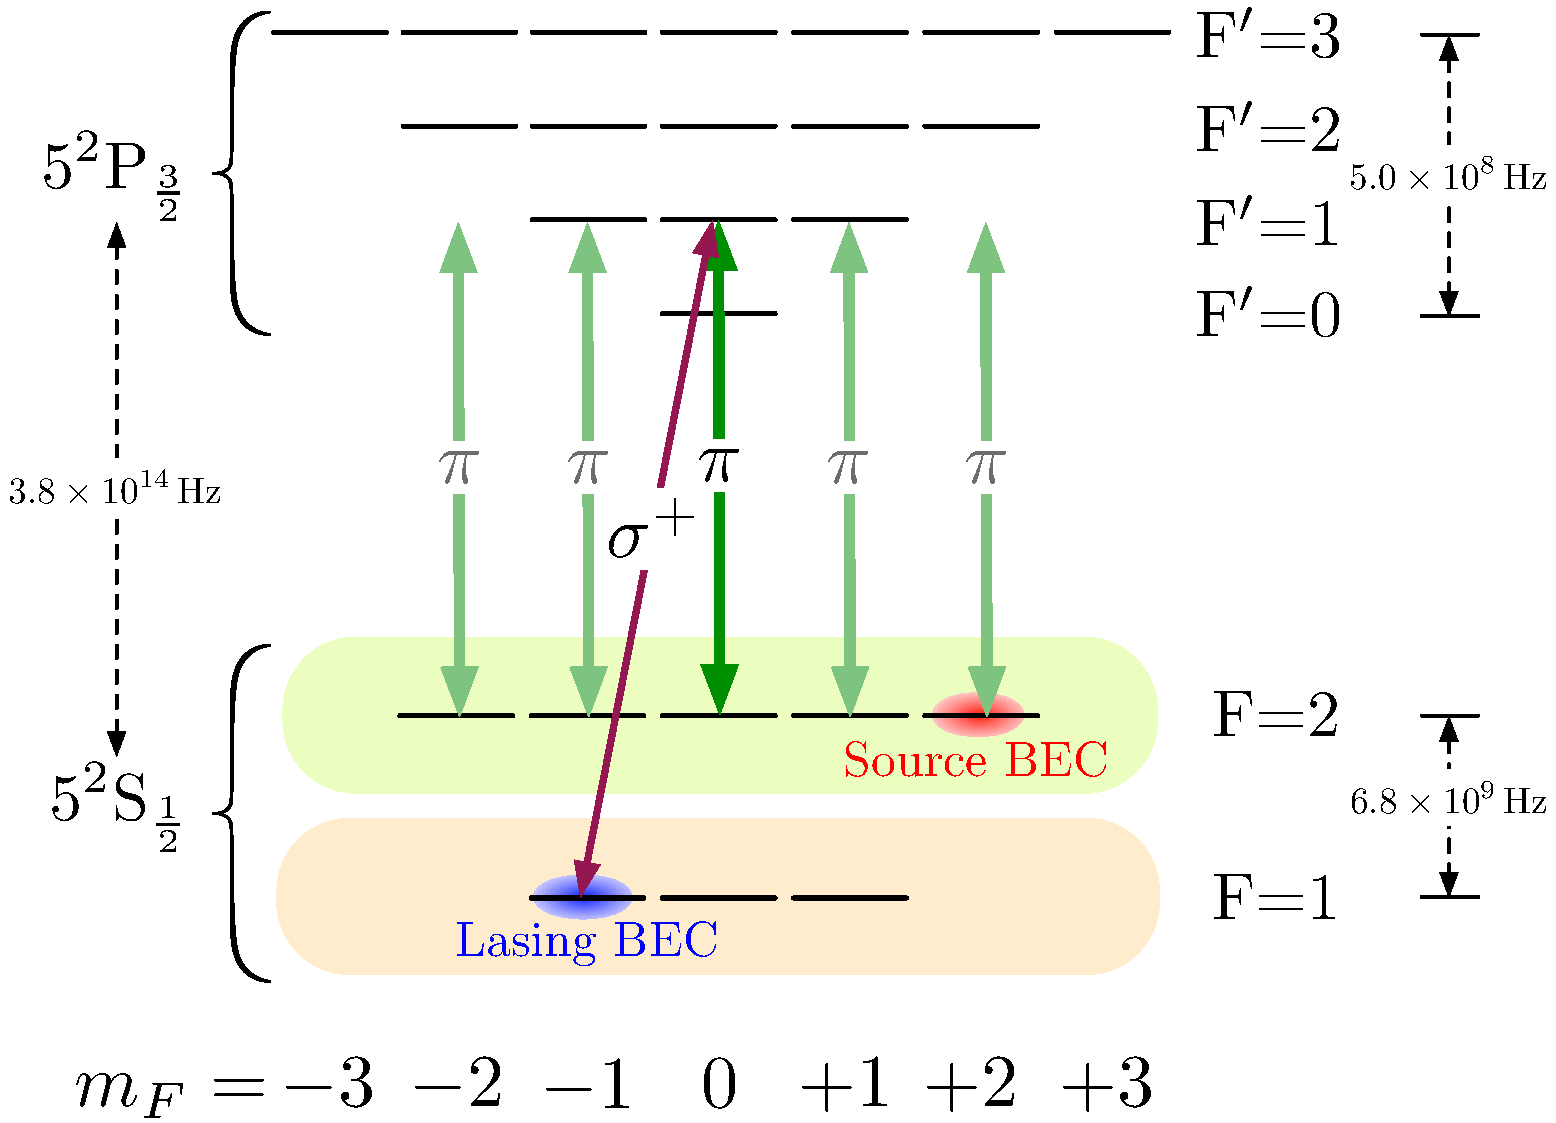
\includegraphics[width=13cm]{LevelDiagram}
    \caption{Level diagram for the continuous pumping experiment.  The $F=2 \leftrightarrow F'=1$ transitions are resonantly driven by $\pi$-polarised optical pumping light.  Although this light couples to several levels, its purpose is to drive $\ket{F=2, m_F=0}$ atoms into the $\ket{F'=1, m_F=0}$ state from which they may be stimulated to decay into the lasing BEC in the $\ket{F=1, m_F=-1}$ state and emit $\sigma^+$-polarised light.}
    \label{OpticalPumping:LevelDiagram}
\end{figure}

Although our aim is to model the continuous pumping experiment described in \sectionref{OpticalPumping:ContinuousExperiment}, we also wish to be able to consider the limit in which the pumping light is significantly detuned (by several GHz).  In either case, the only relevant optical transitions are those in the $\text{D}_2$ line (those pictured in \figureref{OpticalPumping:LevelDiagram}) as all other levels are sufficiently detuned to be negligibly populated.  The transitions closest in frequency to the $\text{D}_2$ line are those of the $\text{D}_1$ line which are detuned by $7 \times \unit[10^{12}]{Hz}$, significantly greater than the maximum expected detuning from the $\text{D}_2$ line.


\subsection{Model derivation}
\label{OpticalPumping:MultimodeModelDerivation}

We begin with the Hamiltonian for the combined atom--light system,
\begin{subequations}
    \label{OpticalPumping:AtomLightHamiltonian}
    \begin{align}
        \hat{H} &= \hat{H}_\text{atoms} + \hat{H}_\text{light} + \hat{H}_\text{atoms--light}, \\
        \begin{split}
            \hat{H}_\text{atoms} &= \sum_i \int d \vect{x}\, \hat{\Psi}_i^\dagger(\vect{x}) \left[ - \frac{\hbar^2 \nabla^2}{2 M} + V_i(\vect{x}) \right] \hat{\Psi}_i(\vect{x}) \\
            &\relphantom{=} + U \sum_{ij}\int d \vect{x}\, \hat{\Psi}_i^\dagger(\vect{x}) \hat{\Psi}_j^\dagger(\vect{x}) \hat{\Psi}_j^{\phantom{\dagger}}(\vect{x}) \hat{\Psi}_i^{\phantom{\dagger}}(\vect{x}),
        \end{split}\\
        \hat{H}_\text{light} &= \sum_\lambda \int d \vect{k}\, \hbar c \abs{\vect{k}} \hat{\Phi}_\lambda^\dagger(\vect{k}) \hat{\Phi}_\lambda(\vect{k}), \\
        \hat{H}_\text{atoms--light} &= - \int d \vect{x}\, \hat{\vect{d}}(\vect{x}) \cdot \hat{\vect{E}}(\vect{x}), \label{OpticalPumping:AtomLightCouplingHamiltonian}
    \end{align}
\end{subequations}
where $\hat{\Psi}_i(\vect{x})$ is the atomic field operator for the internal atomic state $i$, $\hat{\Phi}_\lambda(\vect{k})$ is the field operator for photons of polarisation $\lambda$, the atomic dipole operator is
\begin{align}
    \hat{\vect{d}}(\vect{x}) &= \sum_{ij}\vect{d}_{ij} \hat{\Psi}_i^\dagger(\vect{x}) \hat{\Psi}_j^{\phantom{\dagger}}(\vect{x}),
\end{align}
where $\vect{d}_{ij} = -e\left<i\middle|\vect{r}\middle|j\right> = \vect{d}_{ji}$ is the dipole matrix element\footnote{These matrix elements may all be chosen to be real as by the Wigner-Eckart theorem \citep{Eckart:1930,Brink:1962} all matrix elements within the $\text{D}_2$ line (the levels illustrated in \figureref{OpticalPumping:LevelDiagram}) may be written as real multiples of a reduced dipole matrix element for the $\text{D}_2$ transition.} for the atomic transition $i \leftrightarrow j$, and the electric field operator is given by
\begin{align}
    \hat{\vect{E}}(\vect{x}) &= \sum_\lambda \frac{1}{(2\pi)^{3/2}} \int d \vect{k}\, \left[\unitvec{u}_\lambda(\vect{k}) \left(\frac{\hbar \omega_{\vect{k}}}{2\varepsilon_0} \right)^{\frac{1}{2}} \hat{\Phi}_\lambda(\vect{k}) e^{i \vect{k} \cdot \vect{x}} + \text{h.c.}\right],
\end{align}
where $\unitvec{u}_\lambda(\vect{k})$ is the electric polarisation unit vector for polarisation $\lambda$ (an inverted hat is used to denote unit vectors to avoid confusion with the use of hats for operators).

The Hamiltonian \eqref{OpticalPumping:AtomLightHamiltonian} describes the full dynamics of the system including the spontaneous decay of excited atomic levels.  From this complete description of the system we wish to obtain a simplified model with which we can investigate the behaviour of the experiment described in \sectionref{OpticalPumping:ContinuousExperiment}, and the underlying pumping mechanism more generally.  

The first simplification we will make is to assume that all atomic and optical modes are coherent states, i.e.\  the mean-field approximation.  While this approximation is justified for the condensed atomic fields and the strongly-occupied parts of the optical field (due to the pumping laser and stimulated emission into the lasing BEC), the vacuum fluctuations responsible for spontaneous emission are necessarily neglected by any mean-field model.  The effect of spontaneous emission may be partially included by adding a decay term for the excited atomic levels, however this necessarily neglects the effect of atoms that have undergone spontaneous emission.  While some of these atoms will decay into internal atomic states that are dark to both the optical pumping laser and photons emitted by stimulated emission, others will decay into the same internal atomic level as the target condensate, however with non-zero momentum.  These decays can cause heating if the photon they emit is absorbed by the lasing condensate as some fraction of the atoms that reabsorb these photons will not decay back into the lasing condensate. This process is neglected by this treatment of spontaneous emission.  The effect of this approximation is discussed further in \sectionref{OpticalPumping:Discussion}\footnote{FIXME: Cross-ref to unwritten content. Check at a later date.}.

The semiclassical mean-field model for this system is readily obtained from the Heisenberg evolution equations written in normal order,
\begin{subequations}
    \label{OpticalPumping:HeisenbergEvolution}
    \begin{align}
        i \hbar \frac{\partial}{\partial t} \hat{\Psi}_i(\vect{x}) &= \left(- \frac{\hbar^2 \nabla^2}{2 M} + V_i(\vect{x}) + U\sum_j\hat{\Psi}_j^\dagger(\vect{x})\hat{\Psi}_j^{\phantom{\dagger}}(\vect{x})\right)\hat{\Psi}_i(\vect{x}) - \sum_{j} \vect{d}_{ij} \cdot \hat{\vect{E}}(\vect{x}) \hat{\Psi}_j(\vect{x}),\\
        i \hbar \frac{\partial}{\partial t} \hat{\Phi}_\lambda(\vect{k}) &= \hbar c \abs{\vect{k}} \hat{\Phi}_\lambda(\vect{k}) - \left(\frac{\hbar \omega_{\vect{k}}}{2 \varepsilon_0}\right)^{\frac{1}{2}} \unitvec{u}_\lambda^*(\vect{k}) \cdot \left( \frac{1}{\left(2\pi\right)^{3/2}} \int d \vect{x}\, \hat{\vect{d}}(\vect{x}) e^{-i \vect{k} \cdot \vect{x}} \right),
    \end{align}
\end{subequations}
by replacing all operators with their expectation values.  This yields equations identical in form to \eqref{OpticalPumping:HeisenbergEvolution} without the operator hats.

Our next approximation is to neglect the fast-rotating parts of the atom--light coupling terms in \eqref{OpticalPumping:HeisenbergEvolution}, i.e.\  the rotating wave approximation (RWA).  We achieve this by first separating the purely real electric field into positive and negative frequency terms
\begin{align}
    \vect{E}(\vect{x}) &= \vect{E}_+(\vect{x}) + \vect{E}_-(\vect{x}), \\
    \vect{E}_+(\vect{x}) &= \sum_\lambda \frac{1}{(2\pi)^{3/2}} \int d \vect{k}\, \unitvec{u}_\lambda(\vect{k}) \left(\frac{\hbar \omega_{\vect{k}}}{2 \varepsilon_0}\right)^{\frac{1}{2}} \Phi_\lambda(\vect{k}) e^{i \vect{k} \cdot \vect{x}},\\
    \vect{E}^{\phantom{*}}_-(\vect{x}) &= \vect{E}_+^*(\vect{x}) = \sum_\lambda \frac{1}{(2\pi)^{3/2}} \int d \vect{k}\, \unitvec{u}^*_\lambda(\vect{k}) \left(\frac{\hbar \omega_{\vect{k}}}{2 \varepsilon_0}\right)^{\frac{1}{2}} \Phi^*_\lambda(\vect{k}) e^{-i \vect{k} \cdot \vect{x}},
\end{align}
where $\vect{E}_+(\vect{x})$ contains the positive frequency terms rotating as $e^{-i \omega_{\vect{k}} t}$, and $\vect{E}_-(\vect{x})$ contains the negative frequency terms $e^{i \omega_{\vect{k}} t}$.  In order to clarify the application of the RWA, we must separate the atomic fields $\Psi_i$ into ground [denoted with an unprimed index, $\Psi_i(\vect{x})$] and excited [denoted with a primed index, $\Psi_{i'}(\vect{x})$] states.  The RWA is equivalent to retaining only the explicitly energy-conserving terms $\hat{\vect{E}}_+^\dagger(\vect{x})\hat{\Psi}_i^\dagger(\vect{x}) \hat{\Psi}_{j'}(\vect{x})$ (and their Hermitian-conjugates) of the atom--light coupling Hamiltonian \eqref{OpticalPumping:AtomLightCouplingHamiltonian}.  

Making the rotating wave approximation, the equations of motion for the mean-field become
\begin{subequations}
    \label{OpticalPumping:MeanFieldRWAEvolution}
    \begin{align}
        \begin{split}
            i \hbar \frac{\partial}{\partial t} \Psi_i(\vect{x}) &= \left( -\frac{\hbar^2 \nabla^2}{2M} + V_i(\vect{x}) + U \sum_j \abs{\Psi_j(\vect{x})}^2\right) \Psi_i(\vect{x})\\
            &\relphantom{=} - \sum_{j'} \vect{d}_{ij'} \cdot \vect{E}_+^*(\vect{x}) \Psi_{j'}(\vect{x})
        \end{split}\\
        \begin{split}
            i \hbar \frac{\partial}{\partial t} \Psi_{i'}(\vect{x}) &= \left( -\frac{\hbar^2 \nabla^2}{2M} + V_{i'}(\vect{x}) + U \sum_j \abs{\Psi_j(\vect{x})}^2 - \frac{i\hbar \Gamma}{2}\right) \Psi_{i'}(\vect{x})\\
            &\relphantom{=} - \sum_j \vect{d}_{i'j} \cdot \vect{E}_+(\vect{x}) \Psi_j(\vect{x}) 
        \end{split}\\
        \begin{split}
            i \hbar \frac{\partial}{\partial t} \Phi_\lambda(\vect{k}) &= \hbar c \abs{\vect{k}} \Phi_\lambda(\vect{k}) \\
            &\relphantom{=}- \left(\frac{\hbar \omega_{\vect{k}}}{2 \varepsilon_0}\right)^{\frac{1}{2}} \unitvec{u}_\lambda^*(\vect{k}) \cdot \left( \frac{1}{\left(2\pi\right)^{3/2}} \int d \vect{x}\, \sum_{ij'}\vect{d}_{ij'} \Psi^*_i(\vect{x}) \Psi_{j'}(\vect{x}) e^{-i \vect{k} \cdot \vect{x}} \right),
        \end{split}\label{OpticalPumping:MeanFieldPhotonRWAEvolution}
    \end{align}
\end{subequations}
where the damping of the excited atoms due to spontaneous emission at a rate $\Gamma$ has been included, and the density of the excited atoms has been neglected in the $s$-wave interaction terms.

Our next approximation is to recognise that most of the photon modes will be empty; the photon field will only be nonzero near a finite set of wavenumbers $\vect{q}_n$ (for corresponding polarisations $\lambda_n$).  In the case of the experiment described in \sectionref{OpticalPumping:ContinuousExperiment}, only those modes excited by the optical pumping laser or emitted as atoms undergo stimulated transitions into the target condensate will be occupied (see \figureref{OpticalPumping:LevelDiagram}).  There will also be some small range of wavenumbers occupied around each of these due to spatial variations in the strength of these fields.  If we assume that the spatial envelope of each of these occupied modes varies on a length scale much larger than the wavelength (the slowly-varying envelope approximation), then only modes within $\delta k \ll \abs{\vect{q}_n}$ will be significantly occupied.

If all the occupied photon modes $\vect{q}_n$ are separated by more than $\delta k$, the photon and electric field may be decomposed as
\begin{align}
    \Phi_\lambda(\vect{k}) &= \sum_n \delta_{\lambda, \lambda_n} \Phi_{\lambda_n,\vect{q}_n}(\vect{k}), \\
    \vect{E}_+(\vect{x}) &= \sum_n \vect{E}_{+,\vect{q}_n}(\vect{x}),
\end{align}
where $\delta_{ij}$ is the Kronecker delta.

As each of the photon fields $\Phi_{\lambda_n, \vect{q}_n}(\vect{k})$ will only be occupied within a small range of wavenumbers $\delta k$, the photon energy and polarisation vectors can be assumed to differ negligibly from their values at $\vect{k}=\vect{q}_n$. This permits the corresponding electric field components to be written as
\begin{align}
    \vect{E}_{+, \vect{q}_n}(\vect{x}) &= \frac{1}{(2\pi)^{3/2}} \int d \vect{k}\, \unitvec{u}_{\lambda_n} (\vect{k}) \left(\frac{\hbar \omega_{\vect{k}}}{2\varepsilon_0}\right)^{\frac{1}{2}} \Phi_{\lambda_n, \vect{q}_n}(\vect{k}) e^{i \vect{k}\cdot \vect{x}} \notag\\
    &\approx \unitvec{u}_{\lambda_n}(\vect{q}_n) \left( \frac{\hbar \omega_{\vect{q}_n}}{2\varepsilon_0}\right)^{\frac{1}{2}}   \frac{1}{(2\pi)^{3/2}} \int d \vect{k}\, \Phi_{\lambda_n, \vect{q}_n}(\vect{k}) e^{i \vect{k}\cdot \vect{x}}\notag\\
   &= \unitvec{u}_{\lambda_n}(\vect{q}_n) \left( \frac{\hbar \omega_{\vect{q}_n}}{2\varepsilon_0}\right)^{\frac{1}{2}} \Phi_{\lambda_n, \vect{q}_n} (\vect{x}) \notag\\
   &= \unitvec{u}_{\lambda_n}(\vect{q}_n) E_{+, \vect{q}_n}(\vect{x}),
\end{align}
where $\Phi_{\lambda_n, \vect{q}_n}(\vect{x})$ is the inverse Fourier-transform of $\Phi_{\lambda_n, \vect{q}_n}(\vect{k})$, and $E_{+, \vect{q}_n}(\vect{x})$ is defined by
\begin{align}
    E_{+, \vect{q}_n}(\vect{x}) &= \left( \frac{\hbar \omega_{\vect{q}_n}}{2 \varepsilon_0}\right)^{\frac{1}{2}} \Phi_{\lambda_n, \vect{q}_n}(\vect{x}).\label{OpticalPumping:ElectricFieldPhotonFieldRelationship}
\end{align}

To obtain separate evolution equations for each of the $\Phi_{\lambda_n, \vect{q}_n}(\vect{k})$, the contribution of the atomic coupling terms of \eqref{OpticalPumping:MeanFieldPhotonRWAEvolution} to the evolution of $\Phi_\lambda(\vect{k})$ must be split amongst the evolution equations for the $\Phi_{\lambda_n, \vect{q}_n}(\vect{k})$.  If each atomic transition is only energy-resonant with a single optical mode $\vect{q}_n$ (e.g.\ the $\pi$-polarised transition between $\ket{F=2, m_F=0} \leftrightarrow \ket{F'=1, m_F=0}$ illustrated in \figureref{OpticalPumping:LevelDiagram}), the splitting is obvious.  It is however possible that two or more optical modes may be energy resonant with a single atomic transition (the wavenumbers of all resonant modes will have the same magnitude); this case is more complicated.  In this derivation we wish to consider the possibility that an atomic transition might be resonant with two optical modes propagating in opposite directions\footnote{As discussed at the end of \sectionref{OpticalPumping:ContinuousExperiment}, it is unclear in the continuous pumping experiment whether the $\sigma^+$ photons emitted as the atoms are stimulated to emit into the lasing condensate are emitted vertically upwards or downwards.  If both possibilities are allowed, then both the upward- and downward-propagating modes would be energy-resonant with a single atomic transition.  Another case in which two counter-propagating optical modes may be resonant with a single atomic transition is in the Bragg reflection of light by a matter-wave grating.}.  In this case the contribution of the atomic coupling terms may be separated into two halves: the contribution at wavenumbers $\vect{k}$ such that $\vect{q}_n \cdot \vect{k} > 0$ only affecting $\Phi_{\lambda_n, +\vect{q}_n}(\vect{k})$, and the contribution for which $\vect{q}_n \cdot \vect{k} < 0$ only affecting $\Phi_{\lambda_n, -\vect{q}_n}(\vect{k})$.  This separation can be achieved by including the full contribution of the relevant atomic coupling terms in the evolution equations for each of the photon fields $\Phi_{\lambda_n, \vect{q}_n}(\vect{k})$, but defining the fields to be zero when $\vect{q}_n \cdot \vect{k} < 0$.  This is not an additional approximation as it has already been assumed that the photon fields $\Phi_{\lambda_n, \vect{q}_n}(\vect{k})$ are only nonzero within a small range $\abs{\vect{k} - \vect{q}_n}\ll \delta k$.  


We denote the atomic transitions $i \leftrightarrow j'$ coupled to the optical mode $\vect{q}_n$ by the set $T_n$. The equations of motion in terms of the separate electric field components are
\begin{subequations}
    \label{OpticalPumping:MeanFieldRWAEvolutionSeparatedOpticalFields}
    \begin{align}
        \begin{split}
            i \hbar \frac{\partial}{\partial t} \Psi_i(\vect{x}) &= \left( -\frac{\hbar^2 \nabla^2}{2M} + V_i(\vect{x}) + U \sum_j \abs{\Psi_j(\vect{x})}^2\right) \Psi_i(\vect{x})\\
            &\relphantom{=} - \sum_{j',n} \vect{d}_{ij'} \cdot \unitvec{u}^*_{\lambda_n}(\vect{q}_n) {E}_{+,\vect{q}_n}^*(\vect{x}) \Psi_{j'}(\vect{x}),
        \end{split}\\
        \begin{split}
            i \hbar \frac{\partial}{\partial t} \Psi_{i'}(\vect{x}) &= \left( -\frac{\hbar^2 \nabla^2}{2M} + V_{i'}(\vect{x}) + U \sum_j \abs{\Psi_j(\vect{x})}^2 - \frac{i\hbar \Gamma}{2}\right) \Psi_{i'}(\vect{x})\\
            &\relphantom{=} - \sum_{j,n} \vect{d}_{i'j} \cdot \unitvec{u}_{\lambda_n}(\vect{q}_n) {E}_{+,\vect{q}_n}(\vect{x}) \Psi_{j}(\vect{x}),
        \end{split}\\
        \begin{split}
            i \hbar \frac{\partial}{\partial t} \Phi_{\lambda_n, \vect{q}_n}(\vect{k}) &= \hbar c \abs{\vect{k}} \Phi_{\lambda_n,\vect{q}_n}(\vect{k}) \\
            &\relphantom{=} - \left(\frac{\hbar \omega_{\vect{q}_n}}{2 \varepsilon_0}\right)^{\frac{1}{2}} \unitvec{u}_{\lambda_n}^*(\vect{q}_n) \cdot \left( \frac{1}{\left(2\pi\right)^{3/2}} \int d \vect{x}\, \sum_{\{i,j'\}\in T_n}\vect{d}_{ij'} \Psi^*_i(\vect{x}) \Psi_{j'}(\vect{x}) e^{-i \vect{k} \cdot \vect{x}} \right), \label{OpticalPumping:MeanFieldSeparatedPhotonEvolution}
        \end{split}
    \end{align}
\end{subequations}
where we have made the same approximations made previously that the electric polarisation vectors and the photon energies vary negligibly for each photon field.

It may seem that we have made an unnecessary complication by separating the single equation of motion for the total photon field \eqref{OpticalPumping:MeanFieldPhotonRWAEvolution} into the set of equations \eqref{OpticalPumping:MeanFieldSeparatedPhotonEvolution} for each significantly occupied mode $\Phi_{\lambda_n, \vect{q}_n}(\vect{k})$. This temporary complication will however enable the equations of motion to be simplified into a form that will be computationally tractable to solve.  In their present form the evolution equations \eqref{OpticalPumping:MeanFieldRWAEvolutionSeparatedOpticalFields} have the problem that the fastest timescale in the problem is that of the propagation of the optical field over the length of the condensate.  For a condensate with a Thomas-Fermi radius of $\sim \unit[20]{\micro m}$, this timescale is $\sim \unit[10^{-13}]{s}$, which is much shorter than the timescale over which the pumping was observed to occur in the experiment ($\sim \unit[10^{-1}]{s}$)!  Any numerical method used to solve the system \eqref{OpticalPumping:MeanFieldRWAEvolutionSeparatedOpticalFields} must resolve dynamics on the shorter timescale to be accurate, but evolve for long enough to see the transfer of atoms occurring on a much slower timescale.  Our aim in the next part of the derivation is to eliminate all fast timescales in the problem to obtain a set of numerically-tractable equations to model the system.

As the equations of motion for the the atomic fields are written in the position basis, it would be convenient to write the equation of motion for the photon fields in the same basis.  To simplify this process it is first necessary to approximate the wavenumber magnitude $\abs{\vect{k}}$ appearing in \eqref{OpticalPumping:MeanFieldSeparatedPhotonEvolution},
\begin{align}
    \abs{\vect{k}} &= \abs{\vect{q}_n + \delta \vect{k}}\notag\\
    &\approx \sqrt{\abs{\vect{q}_n}^2 + 2 \vect{q}_n \cdot \delta \vect{k}} = \abs{\vect{q}_n} \sqrt{1 + \frac{2 \vect{q}_n \cdot \delta \vect{k}}{\abs{\vect{q}_n}^2}}\notag\\
    &\approx \abs{\vect{q}_n} + \unitvec{q}_n \cdot \delta \vect{k} = \abs{\vect{q}_n} + \unitvec{q}_n \cdot \left(\vect{k} - \vect{q}_n\right)\notag\\
    &= \unitvec{q}_n \cdot \vect{k}.
\end{align}
With this approximation, the inverse Fourier transform of \eqref{OpticalPumping:MeanFieldSeparatedPhotonEvolution} gives
\begin{align}
    i \hbar \frac{\partial}{\partial t} \Phi_{\lambda_n, \vect{q}_n}(\vect{x}) &= -i \hbar c \unitvec{q}_n \cdot \nabla \Phi_{\lambda_n, \vect{q}_n}(\vect{x}) - \left(\frac{\hbar \omega_{\vect{q}_n}}{2\varepsilon_0}\right)^{\frac{1}{2}} \unitvec{u}_{\lambda_n}^*(\vect{q}_n) \cdot \sum_{\{i,j'\} \in T_n} \vect{d}_{ij'} \Psi^*_i(\vect{x}) \Psi_{j'}(\vect{x}). \label{OpticalPumping:PhotonFieldTransport}
\end{align}
In directly taking the inverse Fourier transform of \eqref{OpticalPumping:MeanFieldSeparatedPhotonEvolution} we have neglected to take account of the fact that only the wavenumbers $\vect{k}$ for which $\vect{k} \cdot \vect{q}_n > 0$ may contribute in \eqref{OpticalPumping:PhotonFieldTransport}, instead the contribution at all wavenumbers has been included.  These additional contributions will be $2 \vect{q}_n$ out of momentum-resonance, and will average to zero over half a wavelength.

Using \eqref{OpticalPumping:ElectricFieldPhotonFieldRelationship} the photon field may be eliminated in favour of the electric field giving the equation of motion for the electric field:
\begin{align}
    \frac{1}{c} \frac{\partial}{\partial t} E_{+, \vect{q}_n} (\vect{x}) &= - \unitvec{q}_n \cdot \nabla E_{+, \vect{q}_n}(\vect{x}) + i \frac{\abs{\vect{q}_n}}{2 \varepsilon_0} \unitvec{u}^*_{\lambda_n}(\vect{q}_n) \cdot \sum_{\{i,j'\}\in T_n} \vect{d}_{ij'} \Psi^*_i(\vect{x}) \Psi_{j'}(\vect{x}). \label{OpticalPumping:ElectricFieldEvolution}
\end{align}
This equation has the familiar form of a transport process in the $\unitvec{q}_n$ direction (at speed $c$) with a source term. The propagation of the electric field across the system occurs on a sufficiently short timescale that for the atomic dynamics, the velocity can be approximated to be infinite.  By separating the fast phase rotation of the electric and atomic fields from the slowly-varying envelopes, it becomes possible to neglect the finite propagation time of the electric field in \eqref{OpticalPumping:ElectricFieldEvolution} to obtain a set of algebraic equations for the electric field at a given time.  The next step in this process is to remove the fast phase rotation of these fields.

To remove the fast phase rotation of the electric and atomic envelopes, we define slowly-varying (temporally) fields marked with tildes as
\begin{subequations}
    \label{OpticalPumping:PhaseRotationDefinition}
    \begin{align}
        \Psi_i &= \widetilde{\Psi}_i e^{-i (\omega_i - \Delta_i)t}, \\
        \Psi_{i'} &= \widetilde{\Psi}_{i'} e^{-i (\omega_{i'} - \Delta_{i'}) t}, \\
        E_{+, \vect{q}_n} &= \widetilde{E}_{+, \vect{q}_n} e^{-i \omega_{\vect{q}_n}t},
    \end{align}
\end{subequations}
where $\omega_i$ (and $\omega_{i'}$) are the frequencies of the atomic levels (including mean-field shifts), $\Delta_i$ (and $\Delta_{i'}$) are the detunings of those levels.  The definitions of these detunings are illustrated in \figureref{OpticalPumping:PhaseRotationDefinition}.

\begin{figure}
    \centering
    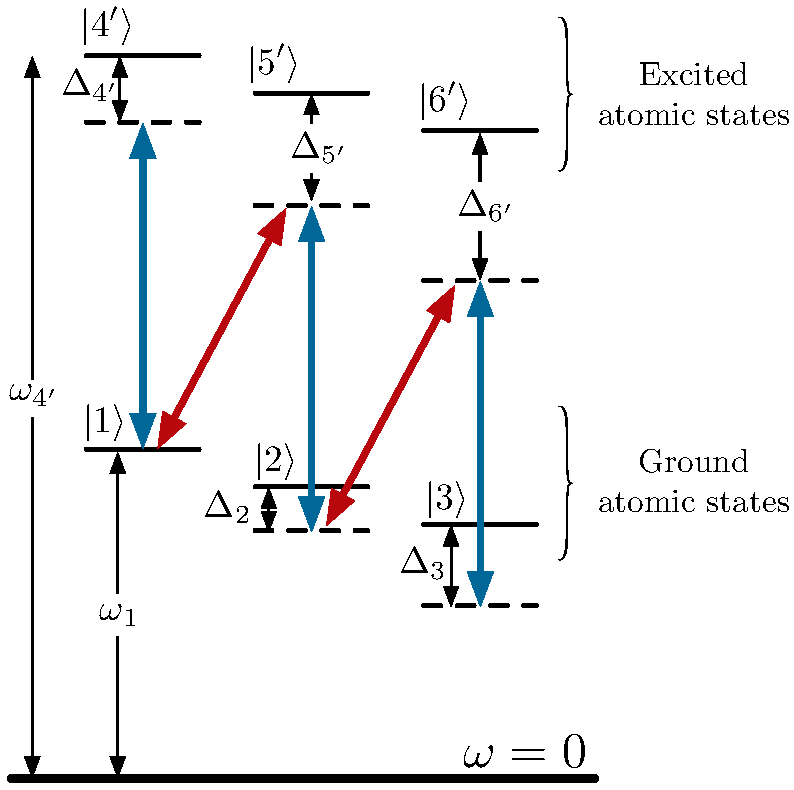
\includegraphics[width=6cm]{PhaseRotationDefinition}
    \caption{Schematic level diagram illustrating the definitions of the detunings in \eqref{OpticalPumping:PhaseRotationDefinition}. The sign of all detunings illustrated are positive.}
    \label{OpticalPumping:PhaseRotationDefinition}
\end{figure}

The equations of motion for the slowly-varying fields are
\begin{subequations}
    \label{OpticalPumping:MeanFieldTemporallySlowlyVarying}
    \begin{align}
        \begin{split}
            i \hbar \frac{\partial}{\partial t} \widetilde{\Psi}_i(\vect{x}) &= \left( -\frac{\hbar^2 \nabla^2}{2M} + V_i(\vect{x}) + U \sum_j \abs{\widetilde{\Psi}_j(\vect{x})}^2 - \hbar \omega_{i} + \hbar \Delta_i \right) \widetilde{\Psi}_i(\vect{x}) \\
            &\relphantom{=} - \sum_{j',n} \vect{d}_{ij'} \cdot \unitvec{u}^*_{\lambda_n}(\vect{q}_n) \widetilde{E}_{+,\vect{q}_n}^*(\vect{x}) \widetilde{\Psi}_{j'}(\vect{x}) e^{-i \left[\omega_{j'} - \Delta_{j'} - (\omega_i - \Delta_i) - \omega_{\vect{q}_n}\right] t},
        \end{split}\\
        \begin{split}
            i \hbar \frac{\partial}{\partial t} \widetilde{\Psi}_{i'}(\vect{x}) &= \left( -\frac{\hbar^2 \nabla^2}{2M} + V_{i'}(\vect{x}) + U \sum_j \abs{\widetilde{\Psi}_j(\vect{x})}^2 - \frac{i\hbar \Gamma}{2} - \hbar \omega_{i'} + \hbar \Delta_{i'}\right) \widetilde{\Psi}_{i'}(\vect{x})\\
            &\relphantom{=} - \sum_{j,n} \vect{d}_{i'j} \cdot \unitvec{u}_{\lambda_n}(\vect{q}_n) \widetilde{E}_{+,\vect{q}_n}(\vect{x}) \widetilde{\Psi}_{j}(\vect{x})  e^{-i \left[\omega_{j} - \Delta_j - (\omega_{i'} - \Delta_{i'}) + \omega_{\vect{q}_n}\right]t},
        \end{split}\\
        \begin{split}
          \frac{1}{c} \frac{\partial}{\partial t} \widetilde{E}_{+, \vect{q}_n} (\vect{x}) &= - \unitvec{q}_n \cdot \nabla \widetilde{E}_{+, \vect{q}_n}(\vect{x}) + i \abs{\vect{q}_n} \widetilde{E}_{+, \vect{q}_n}(\vect{x})\\
          &\relphantom{=} + i \frac{\abs{\vect{q}_n}}{2 \varepsilon_0} \unitvec{u}^*_{\lambda_n}(\vect{q}_n) \cdot \sum_{\{i,j'\}\in T_n} \vect{d}_{ij'} \widetilde{\Psi}^*_i(\vect{x}) \widetilde{\Psi}_{j'}(\vect{x}) e^{-i \left[\omega_{j'} - \Delta_{j'} -(\omega_i - \Delta_i) - \omega_{\vect{q}_n}\right] t}.
        \end{split}
    \end{align}
\end{subequations}
If the level detunings are chosen such that all optical fields couple resonantly between the `detuned levels' (dotted lines in \figureref{OpticalPumping:PhaseRotationDefinition}), the arguments of the exponential terms in \eqref{OpticalPumping:MeanFieldTemporallySlowlyVarying} will all be zero and the terms themselves will be equal to $1$.  Stated mathematically this requirement is
\begin{align}
    \big(\omega_{j'} - \Delta_{j'}\big) - \big(\omega_i - \Delta_i\big) &= \omega_{\vect{q}_n} \;\forall \; i, j', n : \left\{i, j'\right\} \in T_n.
\end{align}
This requirement is satisfied by the optical pumping scheme (see \figureref{OpticalPumping:LevelDiagram}) as the pumping laser defines the detunings of the $F'$ states relative to the $F=2$ states, and the $\sigma^+$ light generated on the $\ket{F=1, m_F=-1} \leftrightarrow \ket{F'=1, m_F=0}$ transition is formed spontaneously, and will therefore be resonant with the transition from the (possibly detuned) $\ket{F'=1, m_F=0}$ state such that the overall two-photon process $\ket{F=2, m_F=0} \leftrightarrow \ket{F=1, m_F=-1}$ is resonant.

With the evolution equations for the slowly-varying envelopes obtained, we may now work to eliminate effects on the propagation timescale of the electric fields.  To achieve this, we choose an arbitrary electric field $\widetilde{E}_{+, \vect{q}_n}$  and transform our coordinate system according to
\begin{align}
  \vect{x}' &= \vect{x}, \\
  t' &= t - \frac{1}{c} \unitvec{q}_n \cdot \vect{x}.
\end{align}

In the primed coordinates, the propagation equation for $\widetilde{E}_{+, \vect{q}_n}$ is
\begin{align}
    \label{OpticalPumping:ElectricFieldSpatialPropagation}
  \begin{split}
    \unitvec{q}_n \cdot \nabla_{\vect{x}'} \widetilde{E}_{+, \vect{q}_n}(\vect{x}', t') &= i \abs{\vect{q}_n} \widetilde{E}_{+, \vect{q}_n}(\vect{x}', t')\\
    &\relphantom{=} + i \frac{\abs{\vect{q}_n}}{2 \varepsilon_0} \unitvec{u}^*_{\lambda_n}(\vect{q}_n) \cdot \sum_{\{i,j'\}\in T_n} \vect{d}_{ij'} \widetilde{\Psi}^*_i\left(\vect{x}', t(\vect{x}', t')\right) \widetilde{\Psi}_{j'}\left(\vect{x}', t(\vect{x}', t')\right),
  \end{split}
\end{align}
where $\widetilde{E}_{+, \vect{q}_n}$ is written as a function of $(\vect{x}', t')$, while the atomic fields are written as functions of $(\vect{x}, t)$.  Although the primed and unprimed time coordinates are not exactly equal, if the spatial origin is chosen to be in the centre of the condensate then $t(\vect{x}', t') \approx t'$ is a very good approximation.  We can estimate the size of the terms neglected by this approximation by considering the variation in the atomic fields over the time $t'-t$,
\begin{align}
    \widetilde{\Psi}^*_i\left(\vect{x}', t(\vect{x}', t')\right) &= \widetilde{\Psi}^*_i\left(\vect{x}', t' + \frac{1}{c} \unitvec{q}_n \cdot \vect{x} \right), \notag\\
    &\approx \widetilde{\Psi}^*_i(\vect{x}', t') \left(1 + i  \frac{\delta \omega}{c}\unitvec{q}_n \cdot \vect{x} \right),
\end{align}
where the atomic field $\widetilde{\Psi}_{i}$ is assumed to evolve in time as $e^{-i\, \delta\omega\, t}$ for sufficiently small times.  For a condensate of maximum spatial extent $\sim \unit[100]{\micro m}$ and an excitation frequency $\delta \omega\sim \unit[10^5]{rad\,s\textsuperscript{-1}}$ (of the order of the chemical potential; refer to the discussion at the end of \sectionref{Peaks:ElementaryExcitations}), this correction term is of the order of
\begin{align}
    \abs{\delta \widetilde{\Psi} / \widetilde{\Psi}} &\leq \frac{\unit[100]{\micro m} \times \unit[10^{5}]{rad\,s\textsuperscript{-1}}}{3 \times \unit[10^8]{m\,s\textsuperscript{-1}}} \approx 10^{-7}.
\end{align}
Although neglecting this correction term is a zeroth-order approximation, the term being neglected is sufficiently small to make this approximation as good as (or better than) many of the first-order approximations that are made elsewhere in this derivation.  A similar approximation needs to be made in the evolution equations for the atomic fields (written in the unprimed coordinate system), $\widetilde{E}_{+, \vect{q}_n}(\vect{x}, t) \approx \widetilde{E}_{+, \vect{q}_n}(\vect{x}, t')$ with a similarly-sized correction.  

The overall effect of this change of coordinate system has been to neglect the temporal derivative in the evolution equation for the electric field mode $\widetilde{E}_{+, \vect{q}_n}$.  To the same degree of approximation, the temporal derivatives of all other electric field modes may also therefore be neglected.  These approximations made, the equations of motion for the system become
\begin{subequations}
    \begin{align}
        \begin{split}
            i \hbar \frac{\partial}{\partial t} \widetilde{\Psi}_i(\vect{x}) &= \left( -\frac{\hbar^2 \nabla^2}{2M} + V_i(\vect{x}) + U \sum_j \abs{\widetilde{\Psi}_j(\vect{x})}^2 - \hbar \omega_{i} + \hbar \Delta_i \right) \widetilde{\Psi}_i(\vect{x})\\
            &\relphantom{=} - \sum_{j',n} \vect{d}_{ij'} \cdot \unitvec{u}^*_{\lambda_n}(\vect{q}_n) \widetilde{E}_{+,\vect{q}_n}^*(\vect{x}) \widetilde{\Psi}_{j'}(\vect{x}),
        \end{split}\\
        \begin{split}
            i \hbar \frac{\partial}{\partial t} \widetilde{\Psi}_{i'}(\vect{x}) &= \left( -\frac{\hbar^2 \nabla^2}{2M} + V_{i'}(\vect{x}) + U \sum_j \abs{\widetilde{\Psi}_j(\vect{x})}^2 - \frac{i\hbar \Gamma}{2} - \hbar \omega_{i'} + \hbar \Delta_{i'}\right) \widetilde{\Psi}_{i'}(\vect{x})\\
            &\relphantom{=} - \sum_{j,n} \vect{d}_{i'j} \cdot \unitvec{u}_{\lambda_n}(\vect{q}_n) \widetilde{E}_{+,\vect{q}_n}(\vect{x}) \widetilde{\Psi}_{j}(\vect{x}),
        \end{split} \label{OpticalPumping:AtomicExcitedStateEvolution}\\
      \unitvec{q}_n \cdot \nabla \widetilde{E}_{+, \vect{q}_n}(\vect{x}) &= i \abs{\vect{q}_n} \widetilde{E}_{+, \vect{q}_n}(\vect{x}) + i \frac{\abs{\vect{q}_n}}{2 \varepsilon_0} \unitvec{u}^*_{\lambda_n}(\vect{q}_n) \cdot \sum_{\{i,j'\}\in T_n} \vect{d}_{ij'} \widetilde{\Psi}^*_i\left(\vect{x}\right) \widetilde{\Psi}_{j'}\left(\vect{x}\right),
    \end{align}
\end{subequations}
where boundary values for the $\widetilde{E}_{+, \vect{q}_n}$ over a plane perpendicular to $\unitvec{q}_n$ must be specified to complete the system of equations.  With the temporal derivatives of the evolution equations for the electric fields neglected, these equations need to be solved self-consistently at every time point.  When all electric fields are propagating in the same direction, this can be viewed as an initial-value problem propagating in the $\unitvec{q}_n$ direction.  This is not the case in the optical pumping scheme in which optical modes may propagate both upwards and downwards.  However as the electric fields evolve slowly in time, the self-consistent solutions may be found iteratively starting from the solution found for the previous time point.

After eliminating the light propagation timescale from the problem, the next fastest timescale is that of the excited atomic states $\widetilde{\Psi}_{i'}$.  The evolution of these states is dominated either by spontaneous decay at a rate $\Gamma = 2\pi \times \unit[5.9]{MHz}$ or by the detuning term (if the pumping laser is detuned by several linewidths).  As these frequencies are much higher than the slower atomic evolution we are interested in ($\sim\unit[10]{kHz}$), the excited states may be adiabatically eliminated.  

To adiabatically eliminate the excited atomic states, we first recognise that the $\hbar \omega_{i'}$ term in \eqref{OpticalPumping:AtomicExcitedStateEvolution} will approximately balance the kinetic, potential and mean-field terms.  With this cancellation made, the adiabatic elimination of the excited atomic states can be made by setting the temporal derivative to zero yielding
\begin{align}
    \widetilde{\Psi}_{i'}(\vect{x}) &\approx \sum_{j, n} \frac{ \vect{d}_{i' j}\cdot \unitvec{u}_{\lambda_n}(\vect{q}_n) \widetilde{E}_{+, \vect{q}_n}(\vect{x}) \widetilde{\Psi}_j(\vect{x})}{\hbar \Delta_{i'} - \frac{i \hbar}{2}\Gamma}.
\end{align}
Substituting this expression back into the remaining evolution equations gives
\begin{subequations}
    \label{OpticalPumping:GeneralMultimodeModel}
    \begin{align}
        \begin{split}
            i \hbar \frac{\partial}{\partial t} \widetilde{\Psi}_i(\vect{x}) &= \left( -\frac{\hbar^2 \nabla^2}{2M} + V_i(\vect{x}) + U \sum_j \abs{\widetilde{\Psi}_j(\vect{x})}^2 - \hbar \omega_{i} + \hbar \Delta_i \right) \widetilde{\Psi}_i(\vect{x})\\
            &\relphantom{=} - \sum_{\substack{j',n\\ l,m}}  \frac{ \left[\vect{d}_{ij'} \cdot \unitvec{u}^*_{\lambda_n}(\vect{q}_n) \right]\left[\vect{d}_{j'l} \cdot \unitvec{u}_{\lambda_m}(\vect{q}_m)\right] }{\hbar \Delta_{j'} - \frac{i \hbar}{2}\Gamma} \widetilde{E}_{+,\vect{q}_n}^*(\vect{x}) \widetilde{E}^{\phantom{*}}_{+, \vect{q}_m}(\vect{x}) \widetilde{\Psi}_{l}(\vect{x}),
        \end{split}\\
        \begin{split}
            \unitvec{q}_n \cdot \nabla \widetilde{E}_{+, \vect{q}_n}(\vect{x}) &= i \abs{\vect{q}_n} \widetilde{E}_{+, \vect{q}_n}(\vect{x}) \\
            &\relphantom{=} + i \frac{\abs{\vect{q}_n}}{2 \varepsilon_0} \sum_{\substack{\{i,j'\}\in T_n\\ l, m}} \frac{\left[\vect{d}_{ij'}\cdot\unitvec{u}^*_{\lambda_n}(\vect{q}_n)\right] \left[\vect{d}_{j' l}\cdot \unitvec{u}_{\lambda_m}(\vect{q}_m)\right] }{\hbar \Delta_{j'} - \frac{i \hbar}{2}\Gamma}  \widetilde{\Psi}^*_i(\vect{x}) \widetilde{\Psi}_l(\vect{x}) \widetilde{E}_{+, \vect{q}_m}(\vect{x}).
        \end{split}
    \end{align}
\end{subequations}
This set of equations represents the basic multimode model that will be used in the remainder of this chapter.

FIXME: Probably need a little more discussion of this model, but that's it.

\parasep

Let us now summarise the approximations and the regimes of validity of the model \eqref{OpticalPumping:GeneralMultimodeModel}.

And we are just about done now.  Write out some polarisation vectors, and then that's it.  We do it all in 1D... oh crap. I forgot about that bit.  Deal with that bit later. This is the full 3D model, then consider 1D systems, then apply the other stuff.

Steps remaining (should be discussed when we apply the model to the optical pumping experiment):
\begin{itemize}
    \item 1D
    \item Polarisation --- atomic vs. optical ($\unitvec{u}_{\pm1} = \frac{1}{\sqrt{2}}\left(\unitvec{x} \pm i \unitvec{y}\right)$, $\unitvec{u}_0 = \unitvec{z}$).
\end{itemize}

In the following sections the multimode pumping model \eqref{OpticalPumping:GeneralMultimodeModel} will be applied to some idealised systems to further investigate the pumping mechanism before applying the model to the pumping experiment itself.

\subsection{Two overlapping condensates model}
\label{OpticalPumping:SimpleModels:OverlappingCondensatesModel}

\begin{figure}
    \centering
    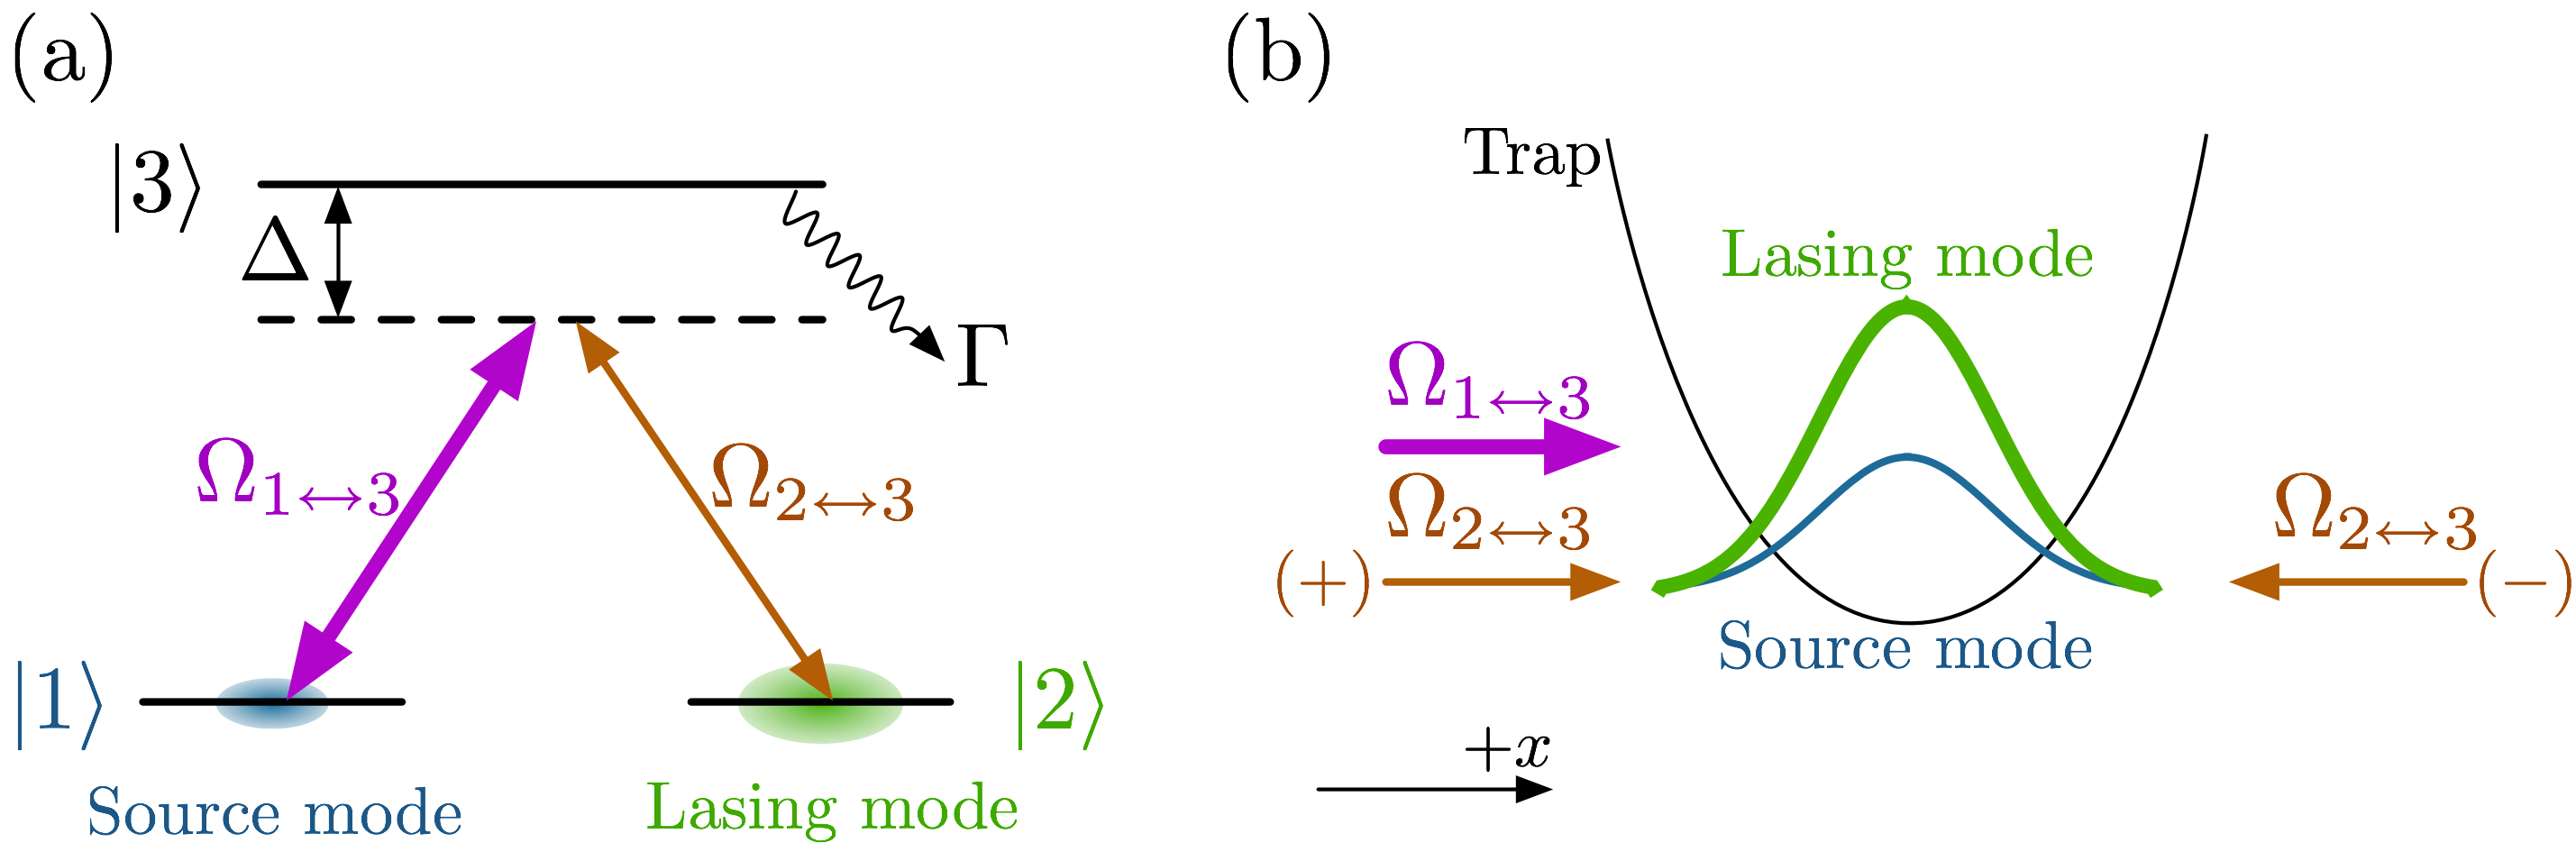
\includegraphics[width=14cm]{OverlappingCondensateModel}
    \caption{Schematic of the two overlapping condensates model.  The system consists of two condensates in the two ground states of a $\Lambda$ level scheme (a).  The system is illuminated on the $\ket{1}\leftrightarrow\ket{3}$ transition by light at a detuning $\Delta$ and Rabi frequency $\Omega_1$.  Light on the $\ket{2} \leftrightarrow \ket{3}$ transition is generated as atoms in the $\ket{3}$ state are stimulated to emit into the lasing mode $\ket{2}$.  Depending on the relative momenta of the atoms in the source and lasing modes, the light on the $\ket{2} \leftrightarrow \ket{3}$ transition will travel to the left or right.  The `$+$' sign in \eqref{OpticalPumping:OverlappingCondensatesEvolution:Omega2} corresponds to the optical field $\Omega_2$ propagating to the right [marked with $(+)$], while the `$-$' sign corresponds to propagation to the left [marked with $(-)$].}
    \label{OpticalPumping:OverlappingCondensateModel}
\end{figure}

The first idealised (multimode) pumping model to be considered is a simplified model of the transfer process occurring at the centre of the lasing condensate in the continuous pumping experiment.  In this model, illustrated in \figureref{OpticalPumping:OverlappingCondensateModel}, the source and lasing modes are the two ground states ($\ket{1}$ and $\ket{2}$ respectively) of atoms with a $\Lambda$-level scheme.  Light on the $\ket{1} \leftrightarrow \ket{3}$ transition is applied with detuning $\Delta$ from the left with an initial Rabi frequency of $\Omega_1(-\infty)$.  Light on the $\ket{2} \leftrightarrow \ket{3}$ transition is not supplied externally but may be produced as a result of atoms in the excited state ($\ket{3}$) being stimulated to emit into the lasing mode ($\ket{2}$).  To investigate possible differences in behaviour if the two optical modes are co-propagating or counter-propagating, we will consider both the case in which the source mode is initially stationary (with the $\Omega_2$ mode propagating to the right) and moving to the left with momentum $2 \hbar k$ (with the $\Omega_2$ mode propagating to the left).  In both cases the initial condition is chosen such that the lasing and source modes are in the overall ground state of the system given their respective initial occupations $N_\text{lasing}(t=0)$ and $N_\text{source}(t=0)$ (i.e.\  in the absence of any optical coupling the system would remain static).  The source mode is assumed to be given its momentum kick to the left (if appropriate) immediately before the optical field $\Omega_1$ is turned on at $t=0$.  As the $\Omega_2$ light is generated by (atomic) stimulated emission its phase will be determined by the phase difference between the source and lasing modes, we may assume there to be a specific phase relationship between the two modes without loss of generality; our results will also apply if the two condensates were independently produced and had a random relative phase.

For the 1D scheme presented in \figureref{OpticalPumping:OverlappingCondensateModel} we may simplify the multimode equations \eqref{OpticalPumping:GeneralMultimodeModel} to
\begin{subequations}
    \label{OpticalPumping:OverlappingCondensatesEvolution}
    \begin{align}
        \begin{split}
            i \hbar \frac{\partial}{\partial t} \Psi_1(x) &= \left[- \frac{\hbar^2}{2M}\frac{d^2}{dx^2} + V_\text{trap}(x) + U_\text{1D}\left(\abs{\Psi_1}^2 + \abs{\Psi_2}^2\right)  \right] \Psi_1\\
            &\relphantom{=} - \hbar \frac{\abs{\Omega_1}^2\Psi_1 + \Omega_1^* \Omega_2^{\phantom{*}}\Psi_2}{\Delta - \frac{i}{2} \Gamma},
        \end{split} \label{OpticalPumping:OverlappingCondensatesEvolution:Psi1}\\
        \begin{split}
            i \hbar \frac{\partial}{\partial t} \Psi_2(x) &= \left[- \frac{\hbar^2}{2M}\frac{d^2}{dx^2} + V_\text{trap}(x) + U_\text{1D}\left(\abs{\Psi_1}^2 + \abs{\Psi_2}^2\right)  \right] \Psi_2\\
            &\relphantom{=} - \hbar \frac{\abs{\Omega_2}^2 \Psi_2 + \Omega_2^* \Omega_1^{\phantom{*}} \Psi_1}{\Delta - \frac{i}{2} \Gamma},
        \end{split} \label{OpticalPumping:OverlappingCondensatesEvolution:Psi2}\\
        \frac{d}{dx} \Omega_1 &= i k \Omega_1 + \frac{i}{4} f_{13} \Gamma \frac{\sigma_0}{A_\perp} \frac{\abs{\Psi_1}^2 \Omega_1 + \Psi_1^* \Psi_2^{\phantom{*}}\Omega_2}{\Delta - \frac{i}{2} \Gamma}, \label{OpticalPumping:OverlappingCondensatesEvolution:Omega1}\\
        \pm \frac{d}{dx} \Omega_2 &= i k \Omega_2 + \frac{i}{4} f_{23} \Gamma \frac{\sigma_0}{A_\perp} \frac{\abs{\Psi_2}^2 \Omega_2 + \Psi_2^* \Psi_1^{\phantom{*}} \Omega_1}{\Delta - \frac{i}{2} \Gamma}, \label{OpticalPumping:OverlappingCondensatesEvolution:Omega2}
    \end{align}
\end{subequations}
where the electric fields of \eqref{OpticalPumping:GeneralMultimodeModel} have been replaced with Rabi frequencies\footnote{Electric fields must be used in the general case in which a single optical field may couple multiple transitions with different dipole matrix elements.  In the present model each optical field drives only a single transition, enabling the electric fields to be replaced with Rabi frequencies.} using $\hbar \Omega_i = \vect{d}_{i 3} \cdot \unitvec{u}_{\lambda_i} \widetilde{E}_{+, \vect{q}_i}$; the remaining dipole matrix elements have been eliminated in favour of the spontaneous emission rate using $\displaystyle \Gamma = \frac{\omega^3 d_\text{total}^2}{3 \pi \epsilon_0 \hbar c^3}$, where the total dipole matrix element is $\abs{d_\text{total}}^2 = \sum_{i} \abs{\vect{d}_{i3}}^2$ with $\abs{\vect{d}_{i3}}^2 = f_{i3} \abs{d_\text{total}}^2$, where $f_{i3}$ is the fraction of atoms in the $\ket{3}$ state that decay to the $\ket{i}$ state; $\displaystyle\sigma_0 = \frac{3 \lambda^2}{2 \pi}$ is the atomic scattering cross-section; and a very simple dimension reduction scheme has been used: $\Psi_i^\text{(3D)} = \Psi_i^\text{(1D)} / \sqrt{A_\perp}$, $U_\text{1D} = U_\text{3D} / A_\perp$, where $A_\perp$ is a representative area of the condensate perpendicular to the $x$ direction.  The positive sign in \eqref{OpticalPumping:OverlappingCondensatesEvolution:Omega2} applies if the source mode is initially stationary causing the $\Omega_2$ mode to propagate to the right, and the negative sign applies if the source mode is initially moving to the left with momentum $2 \hbar k$ causing the $\Omega_2$ mode to propagate to the left.

Before simulating the system numerically, some analytical insight can be obtained by considering the behaviour of the optical fields as they propagate through the condensates.  Although propagating in space instead of in time, the equations of motion for the optical fields resemble those for a coupled $\Lambda$ level scheme with the \emph{atomic} fields governing the strength of the coupling of each transition, a role normally filled by optical fields.  Rewriting the evolution equations for the two optical fields elucidates this analogy,
\begin{subequations}
    \label{OpticalPumping:OpticalPropagationAnalogy}
    \begin{align}
        i \hbar c \frac{d}{dx} \phi_1 &= -\hbar \omega \phi_1  - \hbar \frac{\abs{\Omega_\text{source}}^2 \phi_1 + \Omega_\text{source}^* \Omega_\text{lasing}^{\phantom{*}} \phi_2}{\Delta - \frac{i}{2} \Gamma},\\
        \pm i \hbar c\frac{d}{dx} \phi_2 &= - \hbar \omega \phi_2 - \hbar \frac{\abs{\Omega_\text{lasing}}^2 \phi_2 + \Omega_\text{lasing}^* \Omega_\text{source}^{\phantom{*}} \phi_1}{\Delta - \frac{i}{2} \Gamma},
    \end{align}
\end{subequations}
where $\displaystyle\Omega_\text{source, lasing} = \sqrt{\frac{c \Gamma \sigma_0}{8 A_\perp}} \Psi_{1,\, 2}$, $\phi_i$ has been used to replace the optical Rabi frequencies $\Omega_i$ to limit the possibility for confusion, and it has been assumed that the two optical transitions are of equal strength, hence $f_{13} = f_{23} = \frac{1}{2}$.  The coupling terms between the two fields $\phi_1$ and $\phi_2$ are now clearly in the same form as the atomic coupling terms between $\Psi_1$ and $\Psi_2$ in \eqref{OpticalPumping:OverlappingCondensatesEvolution:Psi1}--\eqref{OpticalPumping:OverlappingCondensatesEvolution:Psi2}.  This similarity is not surprising as the ground state atomic fields and the optical fields may be interchanged in the atom--light coupling Hamiltonian (after making the rotating-wave approximation) without changing its form:
\begin{align}
    \hat{H}_\text{atom--light} &\propto \hat{\Psi}_e^\dagger \hat{\Psi}_g^{\phantom{\dagger}} \hat{\phi} + \hat{\phi}^\dagger \hat{\Psi}_g^\dagger \hat{\Psi}_e^{\phantom{\dagger}},
\end{align}
where $\hat{\Psi}_e$, $\hat{\Psi}_g$ are the excited and ground atomic fields respectively and $\hat{\phi}$ is the photon field.

\begin{figure}
    \centering
    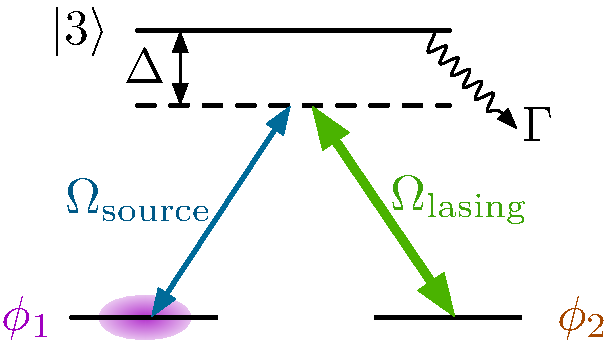
\includegraphics[width=6cm]{DualModel}
    \caption{The propagation of the photons through the system is analogous to Rabi flopping between two states in a $\Lambda$-level scheme.  The flopping between the two modes is driven by `Rabi frequencies' due to the atomic populations of the source and lasing modes.}
    \label{OpticalPumping:DualModel}
\end{figure}

This analogy for the photon propagation is illustrated in \figureref{OpticalPumping:DualModel}.  In this model the two fields $\phi_1$ and $\phi_2$ are coupled by two Rabi frequencies $\Omega_\text{source}$ and $\Omega_\text{lasing}$ that vary (in space) as the two fields $\phi_i$ evolve (in space).  For the counter-propagating case the analogy is imperfect as one mode propagates forward while the other backward, preventing a direct analogy with propagation in time.  For the co-propagating case however, the analogy is perfect and the optical propagation equations can be solved exactly for small times while the source and lasing modes have the same shape.  The solution for $\Omega_2$ is
\begin{align}
    \Omega_2(x) &= \Omega_1(-\infty) \frac{\Psi_1^{\phantom{*}} \Psi_2^*}{\abs{\Psi_1}^2 + \abs{\Psi_2}^2} \left[\exp \left( i \frac{\Gamma \sigma_0}{8 A_\perp\left(\Delta - \frac{i}{2} \Gamma\right)}\int_{-\infty}^x dx\, \abs{\Psi_1}^2 + \abs{\Psi_2}^2\right) -1 \right].
\end{align}

As every photon that leaves the system in the $\Omega_2$ optical mode corresponds to an atom being transferred into the lasing mode, the net rate of atom transfer will be governed by
\begin{align}
    \abs{\Omega_2(+\infty)}^2 &= \abs{\Omega_1(-\infty)}^2 \frac{N_1}{N} \frac{N_2}{N} \abs{\alpha - 1}^2, \label{OpticalPumping:OverlappingCondensates:Omega2Infinity}
\end{align}
where
\begin{align}
    \alpha &= \exp \left( i \frac{N\Gamma \sigma_0}{8 A_\perp\left(\Delta - \frac{i}{2} \Gamma\right)}\right),
\end{align}
$N_i$ is the number of atoms in the $\ket{i}$ state, and $N = N_1 + N_2$ is the number of atoms in the system.  

The rate of atom transfer into the lasing mode is then
\begin{align}
    \frac{d N_2}{dt} &= \abs{\Omega_2(+\infty)}^2 \frac{8 A_\perp}{\Gamma \sigma_0} \\
     &= \abs{\Omega_1(-\infty)}^2 \frac{8 A_\perp}{\Gamma \sigma_0} \frac{N_1}{N} \frac{N_2}{N} \abs{\alpha - 1}^2. \label{OpticalPumping:OverlappingCondensates:TransferRate}
\end{align}
The rate of atom transfer out of the source mode can be found in a similar way.  From these two rates the efficiency of the pumping process may be obtained,
\begin{align}
    \eta &= \left.\frac{d N_2}{d t} \middle / \left(- \frac{d N_1}{dt}\right)\right. = \frac{N_2 \abs{\alpha - 1}^2}{2 N \left(1 - \Re\{\alpha\}\right) - N_1 \abs{\alpha -1}^2}.
\end{align}

\subsubsection{Zero detuning limit ($\Delta = 0$)}

The continuous pumping experiment described in \sectionref{OpticalPumping:ContinuousExperiment} was operated with the pumping light resonant with the $\ket{F=2, m_F=0} \leftrightarrow \ket{F'=1, m_F=0}$ transition; the transition that is represented by the $\ket{1} \leftrightarrow \ket{3}$ transition in the present model.  It is therefore interesting to consider the zero detuning limit ($\Delta = 0$) as it would apply to the experiment.  Furthermore the the lasing mode (the $\ket{F=1, m_F=-1}$ condensate in the experiment) contains significantly more atoms than the source mode (the atom laser state $\ket{F=2, m_F=0}$), permitting the approximation $N_1 \ll N_2$.  

In these limits the parameter $\alpha$ becomes
\begin{align}
    \alpha &= \exp\left( - \frac{N \sigma_0}{4 A_\perp}\right) \approx \exp(- 121) \approx 0,
\end{align}
where a numerical value for $\alpha$ has been obtained using the experimentally-relevant values $\lambda = \unit[780]{nm}$, $N = 5 \times 10^5$, $A_\perp = 3\times\unit[10^{-10}]{m\textsuperscript{2}}$.  Using $\alpha \approx 0$ the transfer rate and efficiency take the simple forms:
\begin{align}
    \frac{d N_2}{dt} &\approx \abs{\Omega_1(-\infty)}^2 \frac{8 A_\perp}{\Gamma \sigma_0} \frac{N_1}{N_2}, \label{OpticalPumping:OverlappingCondensates:ZeroDetuningTransferRate}\\
    \eta &\approx \frac{N_2}{N + N_2} \approx \frac{1}{2} \label{OpticalPumping:OverlappingCondensates:ZeroDetuningEfficiency}.
\end{align}
As observed in the single-mode model of \sectionref{OpticalPumping:SingleModeModel} [see \eqref{OpticalPumping:SingleModePumpingRateZeroDetuning}], the transfer rate \emph{decreases} as the occupation of the lasing mode increases.  

An interesting difference with the single-mode model however is that the transfer efficiency in this model (for short times) cannot exceed 50\% while the efficiency of the single-mode model approaches 100\% for sufficiently large $N_2$.  This difference can be understood by recognising that the $\Lambda$ level scheme of \figureref{OpticalPumping:DualModel} has a dark eigenstate that does not undergo spontaneous emission as the $\ket{3}$ atomic state contains no population.  The dark eigenstate is
\begin{align}
    \ket{D} &= \frac{1}{\sqrt{\abs{\Psi_1}^2 + \abs{\Psi_2}^2}} \left(\Psi_2 \ket{1 \leftrightarrow 3}- \Psi_1 \ket{2\leftrightarrow 3}\right), \label{OpticalPumping:DarkState}\\
    &= \sqrt{\frac{N_2}{N}} \ket{1 \leftrightarrow 3} - \sqrt{\frac{N_1}{N}} \ket{2 \leftrightarrow 3}
\end{align}
where $\ket{i \leftrightarrow j}$ is the state for the optical mode resonant with the $\ket{i} \leftrightarrow \ket{j}$ transition, and the second equality only applies for short times while the two atomic modes have the same spatial profile (and assuming they have the same phase).  It is only the component that is in the dark state that will propagate through the system; all other components will be absorbed rapidly.  Although the projection of the initial (optical) state $\ket{\Psi_\text{initial}} = \ket{1 \leftrightarrow 3}$ onto the dark state
\begin{align}
    \abs{\braket{D}{\Psi_\text{initial}}}^2 &= \frac{N_2}{N}
\end{align}
may approach 1 arbitrarily, the efficiency only approaches $\frac{1}{2}$,
\begin{align}
    \eta &= \frac{\abs{\braket{2 \leftrightarrow 3}{D} \!\!\braket{D}{\Psi_\text{initial}}}^2}{1 - \abs{\braket{1 \leftrightarrow 3}{D} \!\! \braket{D}{\Psi_\text{initial}}}^2} = \frac{\frac{N_1}{N} \frac{N_2}{N}}{1 - \left(\frac{N_2}{N}\right)^2}, \\
    &= \frac{N_2}{N + N_2} \approx \frac{1}{2},
\end{align}
in agreement with \eqref{OpticalPumping:OverlappingCondensates:ZeroDetuningEfficiency}.

The definition of the dark state \eqref{OpticalPumping:DarkState} suggests a method of improving this efficiency: if the profiles of the source and lasing modes are not the same but instead the $\Omega_1$ pumping beam first encounters atoms in the lasing mode before atoms in the source mode, the initial projection onto the dark state will be perfect.  If the variation of the source and lasing mode densities occurs over length scales significantly larger than the absorption length scale for the non-dark states ($\displaystyle \frac{4 A_\perp}{\sigma_0 \abs{\Psi_2}^2} \sim \unit[60]{nm}$), then the dark state will be followed adiabatically with minimal losses.  This situation will arise naturally at later times as the source atoms closest to the pumping beam are transferred to the lasing mode.  As this occurs, the pumping beam will encounter a greater proportion of atoms in the lasing mode than at earlier times thus increasing the efficiency.  This behaviour is observed numerically in simulations of the system \eqref{OpticalPumping:OverlappingCondensatesEvolution} as illustrated in \figureref{OpticalPumping:OverlappingCondensatesZeroDetuning}.

\begin{figure}
    \centering
    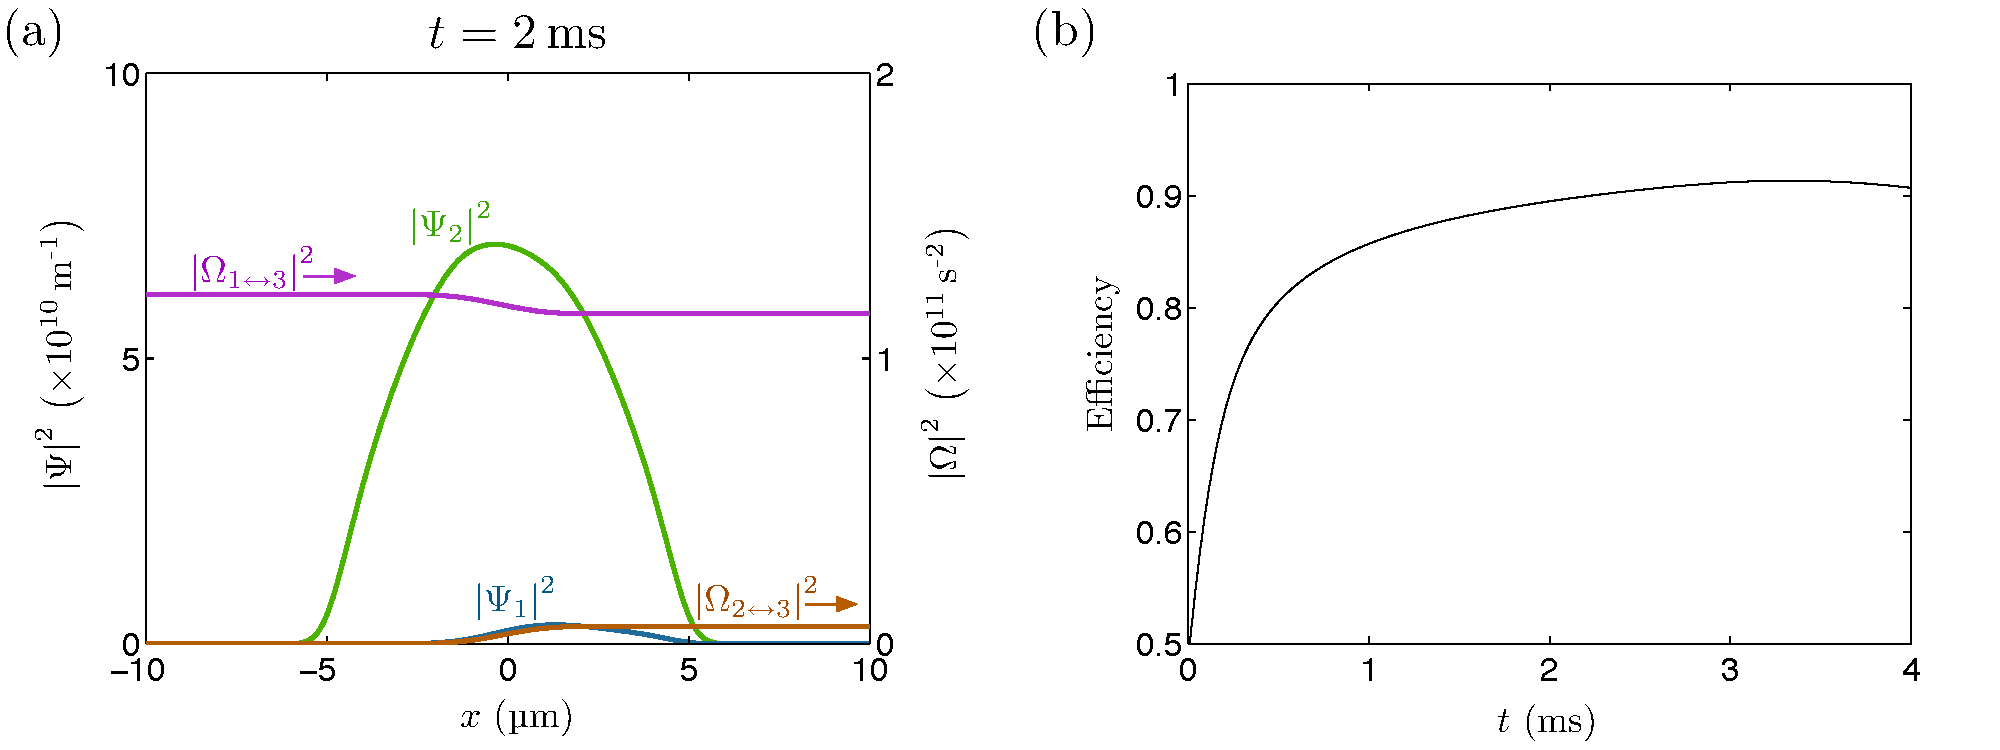
\includegraphics[width=15cm]{OverlappingCondensatesZeroDetuning}
    \caption{Simulation results of the two overlapping condensates model \eqref{OpticalPumping:OverlappingCondensatesEvolution} driven resonantly.  Figure (a) is a snapshot of the densities and magnitudes of the Rabi frequencies at $t = \unit[2]{ms}$.  The instantaneous efficiency is shown in (b).  There are a total of $N = 5 \times 10^5$ atoms in the system, of which initially 5\% are in the source mode ($\ket{1}$), and the system is driven resonantly with $\Omega_1(-\infty) = 3.5 \times \unit[10^5]{s\textsuperscript{-1}}$.}
    \label{OpticalPumping:OverlappingCondensatesZeroDetuning}
\end{figure}

While the efficiency of the population transfer is related to the leading edge of the density profiles, the rate of transfer can be related to the trailing edge.  The fraction of the photons leaving the system in the $\Omega_2$ mode is determined by the dark state at the trailing edge
\begin{align}
    \abs{\Omega_2(+\infty)}^2 &= \abs{\Omega_1(-\infty)}^2 \abs{\braket{2 \leftrightarrow 3}{D_\text{trailing}}\!\! \braket{D_\text{leading}}{\Psi_\text{initial}}}^2, \\
    &= \abs{\Omega_1(-\infty)}^2 \frac{N_1}{N} \frac{N_2}{N},
\end{align}
where the second equality only applies for short times while the two atomic modes have the same spatial profile, and is in agreement with \eqref{OpticalPumping:OverlappingCondensates:Omega2Infinity} as $\alpha \approx 0$.  The rate of population transfer can therefore be increased by having the dark state at the trailing edge to be almost purely the $\ket{2 \leftrightarrow 3}$ state.  This would be achieved by having the density in the lasing mode decay first before the density in the source mode.  In this limit, every photon in the pumping beam would transfer one atom into the lasing mode.  This possibility is related to the idea of adiabatic population transfer \citep{Kuklinski:1989}, and is investigated further in \sectionref{OpticalPumping:SimpleModels:AtomLaserModel}.


This system still suffers from the same problem discussed at the end of \sectionref{OpticalPumping:SingleModeModel}, i.e.\ that the transfer rate is lower than the spontaneous emission rate for atoms that are not momentum resonant with the lasing condensate.  If there is a non-zero time for which the source atoms are not resonant with the lasing condensate (for example, if they must fall from an upper condensate to a lower condensate), this population loss will significantly reduce the overall efficiency of the transfer process.  One possible solution to this problem would be if the pumping process were operated such that every photon in the $\Omega_1$ mode left the system in the $\Omega_2$ mode which the source atoms do not absorb.  This possibility is discussed further in \sectionref{OpticalPumping:SimpleModels:AtomLaserModel}.

\subsubsection{Far detuned limit ($\Delta \gg \Gamma$)}

Although the continuous pumping experiment described in \sectionref{OpticalPumping:ContinuousExperiment} was operated with resonant pumping light, the opposite limit is interesting due to the suppression of spontaneous emission.  In this limit the $\alpha$ parameter becomes
\begin{align}
    \alpha &= \exp\left( - \frac{N \sigma_0}{16 A_\perp} \frac{\Gamma^2}{\Delta^2 + \frac{1}{4}\Gamma^2}\right) \exp \left(i \frac{N \sigma_0}{8 A_\perp} \frac{\Gamma \Delta}{\Delta^2 + \frac{1}{4} \Gamma^2}\right) \\
    &\approx \exp \left( - \frac{N \sigma_0}{16 A_\perp} \frac{\Gamma^2}{\Delta^2}\right) \exp \left(i \frac{N \sigma_0}{8 A_\perp} \frac{\Gamma}{\Delta}\right) \\
    &\approx \exp \left( - 30 \frac{\Gamma^2}{\Delta^2}\right) \exp \left( 61 i \frac{\Gamma}{\Delta} \right) \label{OpticalPumping:FarDetunedLimit:ApproxAlphaNumerical},
\end{align}
where the same values have been used as in the resonant case.  Efficiencies close to unity require the magnitude of $\alpha$ to be close to 1.  While this can be achieved relatively easily (a detuning of a few 10's of linewidths is enough for the experimental parameters), the rate of population transfer depends strongly on the phase of $\alpha$ [see \eqref{OpticalPumping:OverlappingCondensates:TransferRate}].  If the detuning is not sufficiently large to make the phase of $\alpha$ small, the photons will Rabi flop between the $\ket{1 \leftrightarrow 3}$ and $\ket{2 \leftrightarrow 3}$ modes, reducing the rate of transfer into the lasing mode.  In this limit, the transfer rate into the lasing mode averaged over all phases for $\alpha$ is
\begin{align}
    \overline{\frac{d N_2}{dt}} &= \abs{\Omega_1(-\infty)}^2 \frac{16 A_\perp}{\Gamma \sigma_0} \frac{N_1}{N} \frac{N_2}{N} \approx \abs{\Omega_1(-\infty)}^2 \frac{16 A_\perp}{\Gamma \sigma_0} \frac{N_1}{N_2}, \label{OpticalPumping:OverlappingCondensates:IntermediateDetuningTransferRate}
\end{align}
which is twice that in the zero detuning limit \eqref{OpticalPumping:OverlappingCondensates:ZeroDetuningTransferRate}, and hence decreases as the occupation of the lasing mode increases.  The factor of two difference comes from the difference in efficiency: in this case the efficiency is approximately 100\%, while it is 50\% in the zero detuning limit.

The situation is much improved if the pumping light is sufficiently detuned that the phase of $\alpha$ is small.  In the limit
\begin{align}
    \frac{N \sigma_0}{8 A_\perp} \frac{\Gamma}{\Delta} &\ll 1,
\end{align}
the transfer rate is
\begin{align}
    \frac{d N_2}{dt} &\approx \frac{\abs{\Omega_1(-\infty)}^2}{\Delta} \frac{\sigma_0}{8 A_\perp} \frac{\Gamma}{\Delta} N_1 N_2, \label{OpticalPumping:OverlappingCondensates:FarDetuningTransferRate}
\end{align}
with an efficiency
\begin{align}
    \eta &\approx \left(1 + \frac{8 A_\perp}{N \sigma_0}\right)^{-1}.
\end{align}
The transfer rate for very high detunings displays Bose-enhancement as it increases for increasing occupation of the lasing mode.  This is a desirable property for a pumping mechanism, as it means that the highest-occupied mode will undergo more gain than lesser-occupied modes.  

As the transfer rate at high-detunings is Bose-enhanced, the system does not suffer from the same problem with spontaneous emission as exists closer to resonance.  The spontaneous emission rate of source atoms in the absence of the condensate,
\begin{align}
    \left. \frac{d N_1}{dt} \right|_\text{no condensate} &\approx - \frac{\abs{\Omega_1(-\infty)}^2}{\Delta^2}\Gamma N_1,
\end{align}
is significantly lower than the pumping rate in the presence of the lasing mode \eqref{OpticalPumping:OverlappingCondensates:FarDetuningTransferRate},
\begin{align}
    \left. \left. \frac{d N_2}{dt} \right|_\text{pumping} \middle / - \left. \frac{d N_1}{dt} \right|_\text{no condensate} \right. &\approx \frac{N \sigma_0}{8 A_\perp},
\end{align}
where this ratio is $\sim 60$ for the parameters of the continuous pumping experiment.

\subsubsection{Counter-propagating optical modes}
The behaviour of this system in the case that $\Omega_1$ and $\Omega_2$ are counter-propagating is not qualitatively different from that described previously for the co-propagating case.  This is because the pumping beam $\Omega_1$ cannot be significantly reduced by propagating through the system when the source mode is significantly less occupied than the lasing mode ($N_1 \ll N_2$).  After propagating through the system (in the co-propagating case), $\Omega_1$ is
\begin{align}
    \abs{\Omega_1(+\infty)}^2 &= \abs{\Omega_1(-\infty)}^2 \abs{1 + \frac{N_1}{N}\left(\alpha - 1\right)}^2.
\end{align}
For $N_1 \ll N$, $\Omega_1$ changes negligibly propagating through the system and is well approximated by a constant.  Being constant, its propagation direction relative to that of $\Omega_2$ can be expected to have little effect on the system's dynamics.  This is observed in numerical simulations of \eqref{OpticalPumping:OverlappingCondensatesEvolution}.


\subsection{Atom laser model}
\label{OpticalPumping:SimpleModels:AtomLaserModel}

\begin{figure}
    \centering
    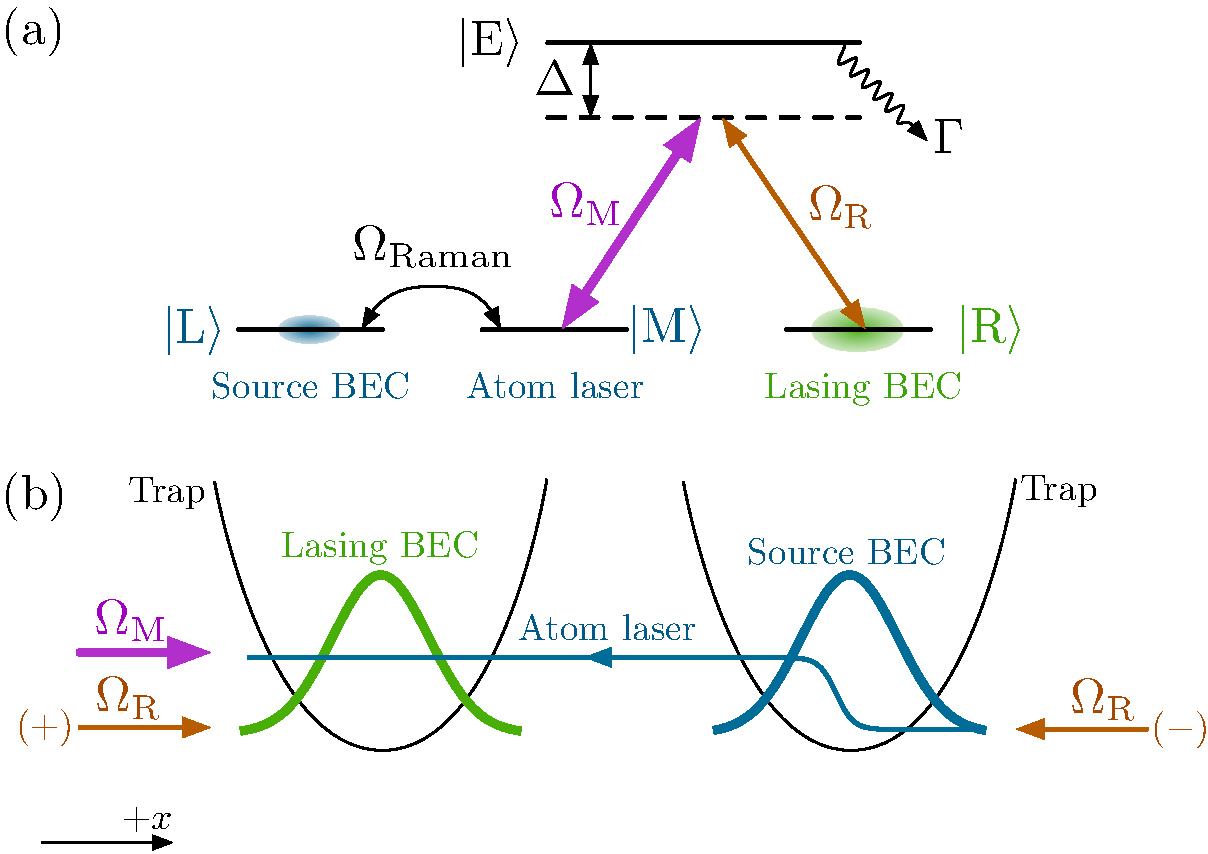
\includegraphics[width=12cm]{TravellingBeamModel}
    \caption{Schematic of the travelling beam model.}
    \label{OpticalPumping:TravellingBeamModel}
\end{figure}



Investigation of the previous model (the overlapping condensates model) suggested that if the source mode were offset from

The second idealised model is much closer to the experimental system.  We have two condensates, we outcouple from one of them to produce an atom laser beam that propagates towards the other and stuff, concrete and ice cream happens for this one.


The equations here are
\begin{subequations}
    \label{OpticalPumping:TravellingBeamEvolution}
    \begin{align}
        \begin{split}
            i \hbar \frac{\partial}{\partial t} \Psi_\text{L}(x) &= \left[ - \frac{\hbar^2}{2M} \frac{d^2}{dx^2} + V_\text{left}(x) + U_\text{1D}\left(\abs{\Psi_\text{L}}^2 + \abs{\Psi_\text{M}}^2 + \abs{\Psi_\text{R}}^2\right) \right] \Psi_\text{R}\\
            &\relphantom{=} +\hbar \Omega_\text{Raman} \Psi_\text{M}
        \end{split}\\
        \begin{split}
            i \hbar \frac{\partial}{\partial t} \Psi_\text{M}(x) &= \left[- \frac{\hbar^2}{2M}\frac{d^2}{dx^2} + U_\text{1D}\left(\abs{\Psi_\text{L}}^2 + \abs{\Psi_\text{M}}^2 + \abs{\Psi_\text{R}}^2\right)  \right] \Psi_\text{M}\\
            &\relphantom{=} + \hbar \Omega^*_\text{Raman} \Psi_\text{L} - \hbar \frac{\abs{\Omega_\text{M}}^2\Psi_\text{M} + \Omega_\text{M}^* \Omega_\text{R}^{\phantom{*}}\Psi_\text{R}}{\Delta - \frac{i}{2} \Gamma},
        \end{split} \label{OpticalPumping:TravellingBeamEvolution:CondensatesEvolution:PsiM}\\
        \begin{split}
            i \hbar \frac{\partial}{\partial t} \Psi_\text{R}(x) &= \left[- \frac{\hbar^2}{2M}\frac{d^2}{dx^2} + V_\text{right}(x) + U_\text{1D}\left(\abs{\Psi_\text{L}}^2 + \abs{\Psi_\text{M}}^2 + \abs{\Psi_\text{R}}^2\right)  \right] \Psi_\text{R}\\
            &\relphantom{=} - \hbar \frac{\abs{\Omega_\text{R}}^2 \Psi_\text{R} + \Omega_\text{R}^* \Omega_\text{M}^{\phantom{*}} \Psi_\text{M}}{\Delta - \frac{i}{2} \Gamma},
        \end{split} \label{OpticalPumping:OverlappingCondensatesEvolution:PsiR}\\
        \frac{d}{dx} \Omega_\text{M} &= i k \Omega_\text{M} + \frac{i}{8} \Gamma \frac{\sigma_0}{A_\perp} \frac{\abs{\Psi_\text{M}}^2 \Omega_\text{M} + \Psi_\text{M}^* \Psi_\text{R}^{\phantom{*}}\Omega_\text{R}}{\Delta - \frac{i}{2} \Gamma}, \label{OpticalPumping:OverlappingCondensatesEvolution:OmegaM}\\
        \pm \frac{d}{dx} \Omega_\text{R} &= i k \Omega_\text{R} + \frac{i}{8} \Gamma \frac{\sigma_0}{A_\perp} \frac{\abs{\Psi_\text{R}}^2 \Omega_\text{R} + \Psi_\text{R}^* \Psi_\text{M}^{\phantom{*}} \Omega_\text{M}}{\Delta - \frac{i}{2} \Gamma}, \label{OpticalPumping:OverlappingCondensatesEvolution:OmegaR}
    \end{align}
\end{subequations}


First we discuss the on-resonance case and mention why it is so fiddly.  Despite this, some meaningful information can be obtained if we take an appropriate time point as a representation of a possible steady-state of the full system.  We will not study the full system.  We get instantaneous efficiency numbers out of this.  We also consider co- and counter-propagating.

Finally, we consider the detuned outcoupling case.

Here we consider co- and counter-propagating models of a double-condensate system with an atom laser as intermediary.  This model is basically Simon's `teleportation' setup. Except backwards.

Results copied from whiteboard:
\begin{itemize}
    \item Co-propagating
    \begin{itemize}
        \item Resonant: Must have $\Phi_\text{photons} > \Phi_\text{atoms}$ for it to work, but this prevents outcoupling.  The next question is whether back-coupling enhances or hinders this. But that is irrelevant.
        \item Detuned: Must avoid Rabi flopping of photons.  Need large intensities.  Highly efficient transfer.
    \end{itemize}
    \item Counter-propagating
    \begin{itemize}
        \item Resonant: Same as co-propagating case
        \item Detuned: ``Flopping due to co-propagation''??? Possibly means atom--light co-propagation?
    \end{itemize}
\end{itemize}


\subsection{3-level model}

\subsection{5-level model}
The 1D model is based on the Maxwell-Schrödinger equations.  One of the technical difficulties is the fact that we must be able to solve in the case that light is travelling in opposite directions simultaneously.  It is not an issue analytically, the equations are well-defined.  The trouble is solving the system self-consistently.  The equations as posed are stiff and are best treated by implicit algorithms, but the best we have are half-arsed semi-implicit algorithms. Better yet would be to use a finite-element method and treat the cross-propagation properly, but I'm lazy.  The other issue is that the frequency of the light is usually known \emph{a priori}.  That is not the case for at least one of the modes in this system.  We therefore need to use some fancy tricks in order to get around that issue.  However, any detunings should not be too large.

Apart from the Maxwell part of the system of equations, everything else is fairly standard.  Except of course for the 1D reduction itself.  We'll call it a `central-line' approximation.

Somewhere in here we need to mention the adiabatic elimination and what kinds of terms it gives rise to.  And in what limit the approximation is valid (even close to resonance).

We need to talk about the other assumptions made in the model.  The assumption that spontaneous emission is negligible.  There is a question about how the 1D approximation affects the Franck-Condon factor, and the relationship between that and spontaneous emission.

Now is a good time to consider $0 \hbar k$ vs $2 \hbar k$ and resonant vs detuned in a simplified model in which things can be controlled (two overlapping modes in the same trap and where $k \rightarrow 0$). The important difference being the \emph{geometry}.

\subsection{3-level model}

This is a simplified model that contains only a small number of levels so that it is easier to keep track of what is going on.  We assume that we can outcouple directly from the $F=2$, $m_F=2$ trapped condensate to the $F=2$, $m_F=0$ state. This isn't realistic, but it is useful to simplify the whole process.  I believe the excited $F'$ manifold was also reduced.  With this simplified model we can investigate resonance vs detuned.  I seem to recall some crazy interesting physics where we had atom transfer back to the \emph{source} condensate in the $0 \hbar k$ configuration in the detuned case.  I believe it was all about phase differences and stuff.  If you look at the equations from the zero-dimensional model, the direction of transfer depends on the phase of a couple of terms, so it can go either way.  For the resonant case, the atoms were definitely transferred to the \emph{target} condensate, as desired.  Also, try as we might, it was not possible to get the $2 \hbar k$ resonance working efficiently.  Too much loss on the way.  Though I don't remember what happened in the detuned $2 \hbar k$ case.

This simplified 1D model contains all of the important physics related to the pumping process.  The delivery of atoms to the target condensate is simplified, and some of the optical transitions are removed.  This model is partly to validate the simple zero-dimensional model including some multimode dynamics, and also to try to get some basic agreement with the experiment before moving on to a more complete description in a later section.

\subsubsection{Comparison with experiment}

We consider both the $0\hbar k$ and the $2\hbar k$ resonance and find that we are able to get reasonable agreement with the experiment in the $0\hbar k$ limit, although it was incredibly fiddly to maximise the transfer.  The $2\hbar k$ resonance was dominated by loss of atoms as they travelled between the source and target condensates.  Although it must be stated that the experimentalists had a good idea of their detunings from rf spectroscopy.  The detunings did indicate that the required conditions for the $0 \hbar k$ resonance were not present.  They were however appropriate for the $2 \hbar k$ resonance, which was the one originally hoped for.  I can't remember, but I wanted to reproduce the experimental rf-spectroscopy data theoretically for some reason.

Anyway, things look great. So why don't we add more realism and see what we get? Maybe we can get even better agreement!

\subsection{5-level model}

The 5-level model is like the 3-level model, but including the full $F=2$ manifold.  Also, the full $F'=1$, $F'=2$ and $F'=3$ excited state manifolds are included before adiabatic elimination.  This model is designed to illustrate the full physics of the situation.  

\subsubsection{Comparison with experiment}

The theory in this case is completely defeated by the crazy mode shape of the $F=2$, $m_F=1$ level.  As this mode is trapped, it oscillates about the lower condensate.  If the intensity of the light is too low, these atoms block the pumping light from even reaching the target condensate and the $F=2$, $m_F=0$ atoms.  If the intensity of the light is too high, the atoms undergo spontaneous emission before they even reach the lower condensate, and you don't get any $F=2$, $m_F=0$ atoms.  If you try for something in the middle, the Franck-Condon factor between the $F=2$, $m_F=0$ atoms and the condensate is very small due to the crazy mode shape of the $F=2$, $m_F=1$ atoms from which the $F=2$, $m_F=0$ atoms are outcoupled.

In short, the 5-level model shows no pumping at all. But not because of something fundamental with the atom transfer process, but rather due to boring technical details about providing the atoms in the appropriate state and mode.  Besides, 1D models are very poor approximations to 5-level systems on timescales beyond the time for the $F=2$, $m_F=1$ atoms to reach the centre of that trap as the atoms will focus at the origin in the tight trapping dimension significantly increasing the density there over what would be seen in a purely 1D model.

\subsection{The pulsed pumping experiment}

The pulsed pumping experiment had the same basic set up as the continuous experiment, but instead a pulse of atoms (the \emph{transfer pulse}) was outcoupled from the upper condensate.  As this pulse was outcoupled over $\unit[100]{\micro s}$ (or whatever time it was) the issue of detuning essentially doesn't arise.  The Fourier width of the outcoupling pulse is large enough to essentially outcouple a copy of the condensate into the different Zeeman levels.  This transfer pulse was allowed to fall a variable delay time before pulsing on the same pumping light used in the continuous experiment.  The transfer pulse was finally allowed to fall further before imaging to determine the number of atoms remaining in the transfer pulse.  Due to the vastly different densities of the condensate and the transfer pulse, it is impossible to simultaneously measure the size of each.  Moreover, as the transfer pulse is significantly smaller than the target condensate, it was impossible to determine the number of transferred atoms to the target condensate.

\subsubsection{Theory / Experiment comparison}

We have good agreement with the loss of atoms out of the transfer pulse, which suggests that the $2 \hbar k$ resonance is workable, although it must be realised that operating a pulsed experiment is fundamentally different to the operation of the continuous experiment.  One model for the operation of the continuous experiment suggests that a process like STIRAP is occurring in the spatial domain instead of the usual temporal domain.  By operating the experiment in the pulsed regime, we are able to cause this process to occur in the temporal domain again, allowing access to the $2 \hbar k$ resonance.  Regardless, there are some questions that remain unanswered.  While we have good agreement on the transfer of atoms \emph{out} of the pulse, the experiment has no information about the transfer of atoms \emph{into} the condensate.  For this question, we can only rely on the theory.  In this case, the theory suggests that there should be a significant number of photons emitted spontaneously within the lower condensate.  A single one of these photons should cause significant (observable) heating of the lower condensate.  The issue is that no such heating is observed.  We are left scratching our heads on this issue (see next section).

\section{Discussion / Outlook}
\label{OpticalPumping:Discussion}

This is where we say that we have reasonable evidence to say that we know what is going on in the transfer of atoms to the lower condensate, but a pretty poor explanation for what happens afterwards.  It is precisely this latter process that was thought to prevent optical pumping of condensates, and so the fact that the expected heating has not been observed is of great interest.  We can speculate wildly as to the origin of this absent heating, including BAR and quantum-mechanical collective effects due to the coherence of the atom laser.  Fundamentally, it seems to me that the notion of spontaneous emission is broken when the emission is occurring in the centre of a BEC.  On the edge, it probably mostly works.  In the centre, I'm not entirely convinced.

\section{Conclusion}

The conclusion I have been thinking of at the moment is along the following lines.  There have been three parts to the optical pumping process: (i) the delivery of atoms in an appropriate state to the condensate being pumped; (ii) the transfer of those atoms to the condensate being pumped; and (iii) the behaviour of the emitted photons within the pumped condensate.  This present chapter has aimed to understand part (ii) of this process.  Ideally we would also like to understand (iii) as it appears that there is some very interesting physics occurring in this part of the process, however we have fallen short of this goal.  By contrast process (i) is a technical detail of getting atoms to the lower condensate with an appropriate mode.  There are several methods that could be used for this process, and there are a number of arguments why the models used in this chapter are unsuitable for fully describing process (i).  Technical details are of course important, but not of fundamental importance.  And it has been the fundamentally important processes that we have aimed to investigate in the present chapter.
